%-------------------------------------------------------------------------------
% THIS FILE IS AN EXAMPLE ON HOW TO USE THE "revstat-v2.sty" PACKAGE...
% last modified: 2019/12/02
%-------------------------------------------------------------------------------
% REVSTAT - STATISTICAL JOURNAL
% Instituto Nacional de Estatística - Portugal
% https://www.ine.pt/revstat/inicio.html
% revstat@ine.pt
%-------------------------------------------------------------------------------
% The following 10 packages are pre-loaded:
%
%     graphicx   latexsym   enumerate   amsmath   amsfonts   amssymb
%     amsthm     amsopn     amstext     amscd     lineno     hyperref
%-------------------------------------------------------------------------------
\documentclass[twoside,leqno,11pt]{article}
\usepackage{revstat-v2}
\usepackage{graphicx, amstext, amsmath, amssymb,color}
\usepackage{siunitx}
\usepackage[colorlinks=true,linkcolor=blue]{hyperref}
\usepackage{subcaption}
\usepackage[a4paper, left=2.5cm, right=2.5cm, top=1.8cm, bottom=1.8cm, includehead, includefoot, head=30pt]{geometry}
\newtheorem{thm}{Theorem}
\usepackage{pdflscape}
%\usepackage{lastpage}
\begin{document}
%%%%%%%%%%%%%%%%%%%%%%%%%% alteracao %%%%%%%%%%%%%%%%%%%%%%%%%%%%%%%%%%
\thispagestyle{firstpage}
\
\vspace{-3.2cm}

\noindent
{\footnotesize {\sffamily REVSTAT~~--~~Statistical~~Journal\\[-1pt]
Volume 0, Number 0, Month 0000,
 000-000}}
% \thepage-\pageref{LastPage}}}   % requires \usepackage{lastpage}

\vspace{1.5cm}
%%%%%%%%%%%%%%%%%%%%%%%%%% alteracao %%%%%%%%%%%%%%%%%%%%%%%%%%%%%%%%%%
%-------------------------------------------------------------------------------
% Title of the article...
%-------------------------------------------------------------------------------
\title{Bias Reduced Peaks over Threshold Tail Estimation}
\renewcommand{\titleheading}
             {Bias Reduced Peaks over Threshold Tail Estimation}  % --- on odd running heads
%-------------------------------------------------------------------------------
% Author(s)' names and addresses...
%-------------------------------------------------------------------------------
\author{\authoraddress{Jan Beirlant \footnote{Corresponding author: Jan Beirlant, KU Leuven, Dept of Mathematics, Celestijnenlaan 200B, 3001 Heverlee,Belgium; Email: jan.beirlant@kuleuven.be} \href{https://orcid.org/0000-0003-0922-6842}{
\includegraphics[scale=0.08]{ORCID-iD_icon-128x128}}}
                      {Department of Mathematics, LStat and LRisk, KU Leuven and\\
                       Department of Mathematical Statistics and Actuarial Science, Free State University\\
                       \texttt{jan.beirlant@kuleuven.be}
                       }
                       
\\
\authoraddress{Gaonyalelwe Maribe \href{https://orcid.org/0000-0002-2795-0909}{
\includegraphics[scale=0.08]{ORCID-iD_icon-128x128}}}
                      {Department of Statistics, University of Pretoria\\
                       \texttt{g.maribe@up.ac.za}}
\\
\authoraddress{Philippe Naveau \href{https://orcid.org/0000-0002-7231-6210}{
\includegraphics[scale=0.08]{ORCID-iD_icon-128x128}}}
                      {Laboratoire des Sciences du Climat et de l'Environnement, CNRS, Universit\'e Paris-Saclay\\
                      \texttt{Philippe.Naveau@lsce.ipsl.fr}}
\\

        \authoraddress{Andr\'{e}hette Verster \href{https://orcid.org/0000-0002-9450-0676}{
\includegraphics[scale=0.08]{ORCID-iD_icon-128x128}}}
                      {Department of Mathematical Statistics and Actuarial Science, Free State University\\
                       \texttt{verstera@ufs.ac.za}}
}
\renewcommand{\authorheading}
             {J.Beirlant, G.Maribe, Ph. Naveau \ and \ A. Verster}  % --- on even running heads

%-------------------------------------------------------------------------------
% Just asking LaTeX to effectively do the title...
%-------------------------------------------------------------------------------
\maketitle
%-------------------------------------------------------------------------------
% Just asking LaTeX to numerate lines...
%-------------------------------------------------------------------------------
\setpagewiselinenumbers
\modulolinenumbers[1]
\linenumbers
%%%%%%%%%%%%%%%%%%%%%%%%%% alteracao: Datas %%%%%%%%%%%%%%%%%%%%%%%%%%%%%%%%%%
\noindent
~~~~{\small{\sffamily Received:} Month 0000 ~~~~~~{\sffamily Revised:} Month 0000 ~~~~~~{\sffamily Accepted:} Month 0000}
%%%%%%%%%%%%%%%%%%%%%%%%%% alteracao %%%%%%%%%%%%%%%%%%%%%%%%%%%%%%%%%%

%-------------------------------------------------------------------------------
% Abstract of the article...
%-------------------------------------------------------------------------------
\begin{abstract}
Bias reduction in tail estimation has mainly been performed in case of Pareto-type models; see  for instance Drees (1996), Peng (1998), Feuerverger and Hall (1999),  Beirlant et al. (1999, 2002), Gomes and Martins (2002) and Caeiro et al. (2005, 2009).  In that context, Beirlant et al. (2009) and Papastathopoulos and Tawn (2013) constructed  distributional models that are based on 
second order rates of convergence for distributions of peaks over thresholds (POT). Such approach also allows to connect  the tail and the bulk of the distribution. 

Bias reduction for all max-domains of attractions, i.e. without restricting to the Pareto-type case, received much less attention up to now. Here we extend the second-order refined POT approach started in Beirlant et al. (2009) providing a bias reduction technique for the classical generalized Pareto (GP) approximation for POTs.
We consider parametric and nonparametric modelling of the second order component. 
\end{abstract}

%-------------------------------------------------------------------------------
% Keywords...
%-------------------------------------------------------------------------------
\begin{keywords}
Peaks over Threshold; Generalized Pareto distribution; Tail estimation; Mixture models.
\end{keywords}

%-------------------------------------------------------------------------------
% AMS classifications...
%-------------------------------------------------------------------------------
\begin{ams}
62G32, 62F10, 62F15, 62J07.
\end{ams}


%-------------------------------------------------------------------------------
% Main text of the paper:  sections, subsections and subsubsections,
%                          with theorems, lemmas, ..., figures, tables, ..., etc
%-------------------------------------------------------------------------------
%%%%%%%%%%%%%%%%%%%%%%%%%% alteracao %%%%%%%%%%%%%%%%%%%%%%%%%%%%%%%%%%
%\mainpaper  % --- just a blank page and a \newpage command
\newpage     % --- just a newpage - not a blank page
%%%%%%%%%%%%%%%%%%%%%%%%%% alteracao %%%%%%%%%%%%%%%%%%%%%%%%%%%%%%%%%%
%-------------------------------------------------------------------------------
% First section
%-------------------------------------------------------------------------------
\section{INTRODUCTION}  % --- sections in UPPERCASE
\label{Sec1}              % --- this section label

\noindent Extreme value (EV) methodology starts from the assumption that the distribution of the available sample $X_1, X_2,\ldots,X_n$ belongs to the domain of attraction of a generalized extreme value distribution, i.e.  there exists sequences $(b_n)_n$ and $(a_n>0)_n$ such that as $n \to \infty$
\begin{equation}
{\max (X_1, X_2,\ldots,X_n)-b_n \over a_n} \to _d Y_{\xi},
\label{maxd}
\end{equation}
where $\mathbb{P} (Y_\xi \leq y) = \exp (-(1+\xi y)^{-1/\xi})$, for some $\xi \in \mathbb{R}$ with $1+\xi y>0$. The parameter $\xi$ is termed the extreme value index (EVI). It is well-known (see e.g. Beirlant et al., 2004, and de Haan and Ferreira, 2006) that \eqref{maxd} is equivalent to the existence of a positive function $t \mapsto \sigma_t$, such that 
\begin{equation}
\mathbb{P}\left({X-t \over \sigma_t} >y| X>t \right)
= {\bar{F}(t+y\sigma_t) \over \bar{F}(t)} \to_{t \to x_+}
\bar{H}^{GP}_{\xi}(y)= (1+\xi y)^{-1/\xi},  
\label{POT}
\end{equation}
where $\bar{F}(x)=\mathbb{P}(X>x)$   and $x_+$ denotes the endpoint of the distribution of $X$. The conditional distribution of $X-t$ given $X>t$ is called the peaks over threshold (POT) distribution, while $\bar{H}_{\xi}^{GP}$ is the survival function of the generalized Pareto distribution (GPD).\\


Estimation of $\xi$ and tail quantities such as return periods is then based on fitting a GPD to the observed excesses $X-t$ given $X>t$.
The main difficulty in such an EV application is the choice of the threshold $t$. Most often, the threshold $t$ is chosen as one of the top data points $X_{n-k,n}$ for some $k \in \{1,2, \ldots,n \}$ where $X_{1,n} \leq X_{2,n} \leq \ldots \leq X_{n,n}$ denotes the ordered sample. 
The parameters $(\xi,\sigma)$ are then estimated by fitting the GPD $H_{\xi}^{GP}\left({y \over \sigma} \right)$ to the spacings $X_{n,n}-X_{n-k,n},\ldots, X_{n-k+1,n}-X_{n-k,n}$.
\\ 


The limit result in \eqref{POT}  requires $t$ to be chosen as large as possible (or, equivalently, $k$ as small as possible) for the bias in the estimation of $\xi$ and other tail parameters to be limited. However, in order to limit the estimation variance, $t$ should be as small as possible, i.e. the number of data points $k$  used in the estimation should be as large as possible. Several adaptive procedures for choosing $t$ or $k$ have been proposed, but mainly in the Pareto-type case with $\xi >0$, i.e. when
\begin{equation}
\bar{F}(x) = x^{-1/\xi}\ell (x),
\label{Patype}
\end{equation} 
for some slowly varying function $\ell$, i.e. satisfying $\frac{\ell(yt)}{\ell (t)} \to 1 $ as $t \to \infty$, for every $y>1$. One then typically assumes a second-order specification of \eqref{Patype} of the type
\begin{equation}
\frac{\ell(yt)}{\ell (t)} - 1 =\delta_t 
\left( y^{-\beta}-1 \right),
\label{SO}
\end{equation}
where $\delta_t=\delta (t)= t^{-\beta}\tilde{\ell}(t)$, with $\beta >0$ and $\tilde\ell$ slowly varying at infinity.
\\

As an alternative, bias reduction techniques  have been proposed in the Pareto-type case $\xi >0$, among others in Feuerverger and Hall (1999),  Beirlant et al. (1999, 2002) and Gomes and Martins (2002). However while the bias is reduced, the variance is increased. In Caeiro et al. (2005, 2009) methods are proposed to limit the variance of bias-reduced estimators  assuming a third-order slow variation model. These methods focus on the distribution of the $\log$-spacings of high order statistics.  Other  construction methods for asymptotically unbiased estimators of $\xi >0$ were introduced in Peng (1998) and Drees (1996).\\
Another approach consists of proposing penultimate limit distributions. In case $\xi >0$, 
Beirlant et al. (2009) proposed an extension of the Pareto distribution (EPD) to approximate the tail probability of the  POT distribution $\mathbb{P}\left( {X \over t}>y|X>t \right)$  as $t \to \infty$:
\begin{equation}
\bar{H}_{\xi,\delta,\rho}^{EP}(y) = 1-H_{\xi,\delta,\rho}^{EP}(y)= y^{-1/\xi}\left( 1+ \delta_t \left( (y^{-1/\xi})^{-\rho}-1\right)\right), \; y>1,
\label{EP}
\end{equation}
with  $\delta_t$ satisfying $\delta_t \downarrow 0$ as $t \to \infty$ and $\rho=-\beta \xi$. In the literature, the second order parameter $\rho$ typically is estimated externally with a different sequence of extreme order statistics than with $\xi$ and $\delta$, or it is given an appropriate 'canonical' value such as -1. We suppress the notation $\rho$ from the extended distribution notation.

Fitting the extended Pareto distribution $H^{EP}_{\xi,\sigma}$ to the relative excesses 
 $\{ {X_{n-j+1,n}\over X_{n-k,n}}, j=1,\ldots,k\}$ leads to estimates of $\xi$ that are more stable as a function of $k$ compared to the original ML estimator derived by Hill (1975)
$$
\hat{\xi}^H_{k,n}= {1 \over k} \sum_{j=1}^k \log {X_{n-j+1,n}\over X_{n-k,n}},
$$
 which is obtained by fitting the Pareto distribution $H^{EP}_{\xi,0}$. Denoting the maximum likelihood estimators of $\xi$ by $\hat{\xi}_k^{EP}$, it can indeed be shown   under the assumption that the EP model for the excesses $X/t$ is correct and that $\rho$ is estimated consistently, that the asymptotic bias of $\hat{\xi}_k^{EP}$ is 0 as long as  $k (k/n)^{-2\rho} \to \lambda \geq 0$ as $k,n \to \infty$, while the asymptotic bias of $\hat{\xi}^H_{k,n}$ is only 0 when $k (k/n)^{-2\rho} \to 0$. On the other hand,  the asymptotic variance of $\hat{\xi}_k^{EP}$ equals $\left({1-\rho\over \rho}\right)^2 {\xi^2 \over k}$, where ${\xi^2 \over k}$ is the asymptotic variance of $\hat{\xi}^H_{k,n}$. 
\\

In case of a real-valued EVI, for the selection of an appropriate threshold or the construction of bias-reduced methods, only a few methods are available. Dupuis (1999) suggested a robust model validation mechanism  to guide the threshold selection, assigning weights between 0 and 1 to each data point where a high weight means that the point should be retained since a GPD model is fitting it well. However, thresholding is required at the level of the weights and hence the method cannot be used in an unsupervised manner. Buitendag et al. (2019) present a ridge regression method to reduce the bias of the generalized Hill estimator proposed in Beirlant et al. (2005). \\

In this paper we concentrate on bias reduction when fitting the GPD  to the distribution of POTs $X-t|X>t$ using maximum likelihood estimation. 
%We apply the flexible semiparametric GP modelling introduced in Tencaliec et al. (2018) to the POT distributions. 
We hence extend the second-order refined POT approach based on $\bar{H}^{EP}_{\xi,\delta}$ from \eqref{EP}  to all max-domains of attraction.
Here the corresponding basic second order regular variation theory can be found in 
Theorem 2.3.8 in de Haan and Ferreira (2006) stating that
 \begin{equation}
 \lim_{t \to x_+}{ \mathbb{P}(X-t >y\sigma_t|X>t)- (1+\xi y)^{-1/\xi} \over \delta (t)} = (1+\xi y)^{-1-1/\xi}\Psi_{\xi,\tilde{\rho}}((1+\xi y)^{1/\xi}),
 \label{secondorder}
 \end{equation}
 with $\delta(t) \to 0$ as $t \to x_+$ and $\Psi_{\xi,\tilde{\rho}}(x)={1 \over \tilde\rho}\left({x^{\xi +\tilde{\rho}}-1 \over \xi +\tilde\rho}- {x^{\xi}-1 \over \xi}\right)$ which for the cases $\xi=0$ and $\tilde\rho=0$ is understood to be equal to the limit as $\xi \to 0$ and $\tilde\rho \to 0$.
We further allow more flexible second-order models than the ones arising from second-order regular variation theory such as in \eqref{secondorder} using non-parametric  modelling of the second-order component and the flexible semiparametric GP modelling introduced in Tencaliec et al. (2019). This  newly proposed method can  also  be applied to the specific case of Pareto-type distributions. 
\\

 In the next section we propose our extended GPD models, and detail the estimation methods. Some basic asymptotic results are provided in section 3. In the final  section we discuss simulation results  and some practical case studies. 


\section{TRANSFORMED AND EXTENDED GPD MODELS}
\label{Sec2}
\noindent
In this paper we propose to  approximate the POT distribution with an extended GPD model with survival function
\[
({\cal{E}}) : \hspace{0.5cm} \bar{F}^{EGP}_t(y)= \bar{H}^{GP}_\xi ({y \over \sigma})\left\{1 +\delta_t B_{\eta} \left( \bar{H}^{GP}_\xi ( {y \over \sigma}) \right) \right\}, 
\]
where 
\begin{itemize}
\item $\delta_t =\delta (t) \to 0$ as $t \to x_+$,
%\item $\delta_t =\delta (t) \uparrow 1$ as $t  \to 0$,
\item $B_{\eta} (1)=0$ and $\lim_{u \to 0} u^{1-\epsilon}B_{\eta}(u)=0$ for every $0<\epsilon <1$,
\item $B_{\eta}$ is twice continously differentiable. 
\end{itemize}
Here the parameter $\eta$ represents a second order nuisance parameter. 
For negative $\delta$-values one needs $\delta_t > \{\min_u (1-{d \over du}\, (uB_{\eta}(u))\}^{-1}$ to obtain a valid distribution. 
\\
Note that this model is a transformation model $G_t \left(\bar{H}^{GP}_\xi ({y \over \sigma}) \right)$ where 
 the transformation function $G_t: (0,1) \to (0,1), u \mapsto  u(1+\delta_t B_{\eta}(u))$ satisfies ${G_t (u) \over u} \to 1$ as $t \to \infty$ for every $u \in (0,1)$ as follows from \eqref{POT}.
 \\
 Also, model ($\cal{E}$)  generalizes the EPD model \eqref{EP} replacing the Pareto survival function $y^{-1/\xi}$ ($\xi >0$) by the GPD survival function $\bar{H}^{GP}_\xi$  ($\xi \in \mathbb{R}$), and considering a general function  $B_\eta (u)$. 
\\
  
\noindent  
We here detail {\it a parametric and non-parametric estimation procedure} for $(\xi,\sigma)$ under $({\cal{E}})$ based on excesses $Y_{j,k}=X_{n-j+1,n}-X_{n-k,n}$ $(j=1,\ldots,k)$, while considering external estimation of the parameters in the $B_{\eta}$ component of the model. In this we use the reparametrization $(\xi,\tau)$ with $\tau=\xi/\sigma$.
Modelling the distribution of the exceedances $Y$ with model ($\cal{E}$) leads to maximum likelihood estimators based on the excesses $Y_{j,k}=X_{n-j+1,n}-X_{n-k,n}$ $(j=1,\ldots,k)$:  
\begin{eqnarray}
(\hat{\xi}^E_k,\hat{\tau}^E_k, \hat{\delta}^E_k)&=&
\mbox{argmax} \left\{
\sum_{j=1}^k \log\left( 
1+\delta_k b_{\eta}((1+\tau Y_{j,k})^{-1/\xi}) \right)
 \right. \nonumber \\
&& \hspace{1.5cm} \left. + \sum_{j=1}^k
\log \{{\tau \over \xi}(1+\tau Y_{j,k})^{-1-1/\xi} \}
%\textcolor{blue}{-\omega {\delta_k^2\over 2 \sigma_{k,n}^2} %
 \right\}
 \label{MLE}
\end{eqnarray}
with $b_{\eta}(u) ={d \over du} (uB_{\eta}(u))$ for a given choice of $B_\eta$.\\
\noindent
Estimates of small tail probabilities $\mathbb{P}(X>c)$ are then  obtained through 
\[
\hat{\mathbb{P}}_k^E(X>c) = {k \over n} \bar{H}^{GP}_{\hat{\xi}^E_k}\left({\hat{\tau}^E_k \over \hat{\xi}^E_k}(c-X_{n-k,n}) \right) 
\left( 1+ \hat{\delta}_k^E \hat{B}_{\eta}\left(\bar{H}^{GP}_{\hat{\xi}^E_k} ({\hat{\tau}^E_k \over \hat{\xi}^E_k}(c-X_{n-k,n})\right)\right).
\]
A general approach to choose the parameters contained in the $B_{\eta}$ component can be to minimize the variance of the obtained estimates of $\xi$ over $k=2,\ldots,n$. See also the simulation section 4.
 
\vspace{0.3cm} \noindent
  {\bf A parametric approach} ($Ep$).  The second-order result \eqref{secondorder} leads to the parametric choice $B_{\xi,\tilde{\rho}}(u)= {u^{\xi} \over \tilde\rho}\left({u^{-\xi -\tilde{\rho}}-1 \over \xi +\tilde\rho}- {u^{-\xi}-1 \over \xi}\right)$ in case  $\xi+\tilde\rho \neq 0$ and $\xi \neq 0$. \\
  Model (${\cal{E}}$)  allows for bias reduction in the estimation of  $(\xi,\tau)$ under the assumption that the corresponding second-order model \eqref{secondorder} is correct for the POTs  $X-t|X>t$. Note that here the $B_{\eta}$ component contains two parameters $\xi$ and $\tilde\rho$. So in this component $\xi$ and $\tilde\rho$ will be substituted with an external value.
  % When model (${\cal E}$)  is used as a model for all observations, i.e. taking $t=0$, this model directly encompasses the models from Frigessi et al. (2002) 	and Naveau et al. (2016).\\
\\
  Here
\[b_\eta (u)= u^{-\tilde\rho}\left( {1-\tilde\rho\over \tilde\rho (\xi +\tilde\rho)}\right)
+ u^\xi \left( {1+\xi \over \xi (\xi +\tilde\rho)}\right)
- {1 \over \xi\tilde\rho},
\]
in which the classical estimator of $\xi$ (with $\delta_k=0$), or an appropriate value $\xi_0$, is used to substitute $\xi$. A consistent estimator of $\tilde\rho$ is provided in Fraga Alves et al. (2003). Another option is to choose  ($\xi_0,\tilde\rho$)  minimizing the variance in the plot of the resulting estimates of $\xi$ as a function of $k$.\\


 \noindent
{\bf A non-parametric approach} ($E{\bar{p}}$). 
In practice a particular distribution probably follows laws of nature, environment or business and does not have to follow the second-order regular variation assumptions as in  \eqref{secondorder}. A non-parametric approximation of $u\mapsto uB_\eta (u)$ can be obtained from an estimator $\hat{G}_{t_*}$ of $G_{t_*}$, or equivalently $\hat{G}_{k_*}$ of $G_{k_*}$, of the transformation $G_t(u)=u(1+\delta_t B_{\eta}(u))$ ($u \in (0,1)$) at some particular $t_*$ or $k_*$.
Indeed, using $\hat{G}_{k_*}^{(m)}(u) -u$ as an approximation of $u \mapsto \delta_{k_*} uB_\eta (u)$, and reparametrizing $\delta_k$ by $\delta_k/\delta_{k_*}$, we obtain $\hat{b}_{\eta,k_*} (u)=-1 + {d \over du}\hat{G}_{k_*}^{(m)}(u)$ as an estimator of $b_\eta$.\\

\noindent
For any $t$, an estimator $\hat{G}_{t}$ of $G_{t}$ can be obtained 
using the Bernstein polynomial  algorithm from Tencaliec et al. (2019). 
The Bernstein approximation of order $m$ of a continuous distribution function $G$ on $[0,1]$
is given by 
\[
G^{(m)}(u) = \sum_{j=0}^m G\left( {j \over m}\right)\left( \begin{array}{c} m \\ j \end{array}\right)u^j (1-u)^{m-j},
\; u \in [0,1].
\]
As in Babu et al. (2002) one then replaces the unknown distribution function $G$ itself with the empirical distribution function $\hat{G}_n$ of the available data in order to obtain a smooth estimator of $G$:
\[
\hat{G}_n^{(m)}(u) = \sum_{j=0}^m \hat{G}_n\left( {j \over m}\right)\left( \begin{array}{c} m \\ j \end{array}\right)u^j (1-u)^{m-j}. 
\] 
Note that $G_t$ is the distribution function of
 $\bar{H}_{\xi}^{GP}(Y/\sigma)$. Hence, in the present application, data from $G_t$ are only available after imputing a value for $(\xi,\tau)$. This then leads to the iterative algorithm from Tencaliec et al. (2019), which is applied to every threshold $t$, or every number of top $k$ data.

\vspace{0.3cm}\noindent
{\small
%{\it Algorithm} ($A_{\cal T}$) 
\begin{enumerate}
\item[(i)] Set starting values ($\hat{\xi}_k^{(0)},\hat{\tau}_k^{(0)}$). Here one can use ($\hat{\xi}_k^{ML},\hat{\tau}_k^{ML}$) from using $G_t (u)=u$.
\item[(ii)]
Iterate for $r=0,1,\ldots$ until the difference in loglikelihood taken in ($\hat{\xi}_k^{(r)},\hat{\tau}_k^{(r)}$) and ($\hat{\xi}_k^{(r+1)},\hat{\tau}_k^{(r+1)}$) is smaller than a prescribed small value:
\begin{enumerate}
\item Given ($\hat{\xi}_k^{(r)},\hat{\tau}_k^{(r)}$)
construct rv's 
$ \hat{Z}_{j,k}= \left( 1+ \hat{\tau}_k^{(r)}Y_{j,k}\right)^{-1/\hat{\xi}_k^{(r)}} 
$
\item Construct Bernstein approximation based on $\hat{Z}_{j,k}$ ($1\leq j \leq k$)
\[
\hat{G}_k^{(m)}(u) = \sum_{j=0}^m \hat{G}_k \left( {j \over m}\right)\left( \begin{array}{c} m \\ j \end{array}\right)u^j (1-u)^{m-j}
\]
with $\hat{G}_k$ the empirical distribution function  of $\hat{Z}_{j,k}$
\item Obtain new estimates ($\hat{\xi}_k^{(r+1)},\hat{\tau}_k^{(r+1)}$) with ML:
\begin{eqnarray*}
(\hat{\xi}_k^{(r+1)},\hat{\tau}_k^{(r+1)})&=&
\mbox{argmax} \left\{
\sum_{j=1}^k \log \{ \hat{g}^{(m)}_k ((1+\tau \hat{Z}_{j,k})^{-1/\xi})\} \right.\\
&& \hspace{1.5cm} \left. + \sum_{j=1}^k
\log \{{\tau \over \xi}(1+\tau \hat{Z}_{j,k})^{-1-1/\xi} \} \right\}
\end{eqnarray*}
with $\hat{g}^{(m)}_k $ denoting the derivative of $\hat{G}_k^{(m)}$.
\end{enumerate}
\end{enumerate}
}

\vspace{0.3cm}\noindent
As noted in Tencaliec et al. (2019) a theoretical study of these estimates is difficult and has not been established. \\ 


\noindent
 {\bf Remark 1.}  The estimation methods described above of course can be rewritten for the specific case of Pareto-type distributions where the distribution of POTs $Y={X \over t}|X>t$ are approximated by transformed Pareto distributions. The model ($\cal{E}$) is then rephrased as 
 \[
({\cal{E}^+}) : \hspace{0.5cm} \bar{F}^E_t(y)= \bar{H}^{P}_\xi (y)\left\{1 +\delta_t B_{\eta} \left( \bar{H}^{P}_\xi (y) \right) \right\}. 
\]
The likelihood estimation method, now based on the exceedances $Y_{j,k}= X_{n-j+1,n}/X_{n-k,n}$ ($j=1,\ldots,k$), is then adapted to
  \begin{equation}
(\hat{\xi}^{E+}_k, \hat{\delta}^{E+}_k)=
\mbox{argmax} \left\{
\sum_{j=1}^k \log\left( 
1+\delta_k b_{\eta}(Y_{j,k}^{-1/\xi}) \right)+
  \sum_{j=1}^k
\log \{{1 \over \xi} (Y_{j,k})^{-1-1/\xi} \}
 \right\}.
\label{E+}
\end{equation}
Note that the ($Ep^+$) approach using the parametric version $B_\eta (u) = u^{-\rho}-1$ for a particular fixed $\rho <0$  equals the EPD method from Beirlant et al. (2009), while ($E\bar{p}^+$) is new. 

\vspace{0.2cm}\noindent
Estimators of tail probabilities are then given  by  
\[
\hat{\mathbb{P}}_k^{E+}(X>c) = {k \over n} \bar{H}^{P}_{\hat{\xi}^{E+}_k}\left( c/X_{n-k,n} \right) 
\left( 1+ \hat{\delta}_k^{E+} \hat{B}_{\eta}\left(\bar{H}^{P}_{\hat{\xi}^{E+}_k} (c/X_{n-k,n})\right)\right).  
\]
%$\Box$ 


\section{BASIC ASYMPTOTICS UNDER MODEL (${\cal E}$)}


In this section we discuss the asymptotic properties of the maximum likelihood estimators solving \eqref{MLE} and \eqref{E+}. To this end, as in Beirlant et al. (2009), we develop the likelihood equations up to linear terms in $\delta_k$ since $ \delta_k \to 0$ with decreasing value of $k$. 
Below we set $\bar{H}_{\theta}(y)=(1+\tau y)^{-1/\xi}$ when using extended GPD modelling, while $\bar{H}_{\theta}(y)=y^{-1/\xi}$ when using extended Pareto modelling under $\xi >0$.

\vspace{0.2cm}\noindent
{\it Extended Pareto POT modelling}. The likelihood problem \eqref{E+} was already considered in Beirlant et al. (2009) in case of  parametric modelling for $B_\eta$. We here propose a more general treatment. The limit statements in the derivation can be obtained using the methods from Beirlant et al. (2009). Denoting the log-likelihood function in \eqref{E+} by $\ell$, the likelihood equations are given by
\begin{equation}
\left\{
\begin{array}{lcl}
{\partial \over \partial \xi} \ell &=&
-{k \over \xi }+ {1 \over \xi^2} \sum_{j=1}^k \log Y_{j,k}
 + {\delta_k \over \xi^2} \sum_{j=1}^k \frac{ b'_\eta (\bar{H}_{\theta}(Y_{j,k}))\bar{H}_{\theta}(Y_{j,k})\log Y_{j,k}}{1+\delta_k b_\eta (\bar{H}_{\theta}(Y_{j,k}))} \\
 {\partial \over \partial \delta_k} \ell &=&
 \sum_{j=1}^k b_\eta (\bar{H}_{\theta}(Y_{j,k}))-\delta_k \sum_{j=1}^k b^2_\eta (\bar{H}_{\theta}(Y_{j,k})).
\end{array}
\right.
\label{systemE+}
\end{equation}

\vspace{0.2cm}\noindent
{\it Extended Generalized Pareto POT modelling}. 
The likelihood equations following from \eqref{MLE} up to linear terms in $\delta_k$ are now given by
\[
\left\{
\begin{array}{lcl}
{\partial \over \partial \xi} \ell &=&
-{k \over \xi }+ {1 \over \xi^2} \sum_{j=1}^k \log (1+\tau Y_{j,k})
 + {\delta_k \over \xi^2} \sum_{j=1}^k  b'_\eta (\bar{H}_{\theta}(Y_{j,k}))\bar{H}_{\theta}(Y_{j,k})\log (1+\tau Y_{j,k}) \\
 {\partial \over \partial \tau} \ell &=&
{k \over \xi \tau}
\left\{ -1+ (1+\xi) {1 \over k}\sum_{j=1}^k {1 \over 1+\tau Y_{j,k}} \right. \\
&& \hspace{1cm} \left. 
 -{\delta_k \over k}\sum_{j=1}^k b'_\eta (\bar{H}_{\theta}(Y_{j,k})) (\tau Y_{j,k}) (1+\tau Y_{j,k})^{-1-1/\xi}
   \right\}
 \\
 {\partial \over \partial \delta_k} \ell &=&
 \sum_{j=1}^k b_\eta (\bar{H}_{\theta}(Y_{j,k}))-\delta_k \sum_{j=1}^k b^2_\eta (\bar{H}_{\theta}(Y_{j,k})),
\end{array}
\right.
\]
from which
\begin{equation}
 \left\{
\begin{array}{l}
\hat{\delta}_k = \frac{\sum_{j=1}^k b_\eta (\bar{H}_{\hat{\theta}_k}(Y_{j,k}))}{\sum_{j=1}^k b^2_\eta (\bar{H}_{\hat{\theta}_k}(Y_{j,k}))}, \\
{1 \over k}\sum_{j=1}^k \log (1+\hat{\tau}_k Y_{j,k})
= \hat{\xi}_k- 
{\hat{\delta}_k \over k}\sum_{j=1}^k b'_{\eta}(\bar{H}_{\hat{\theta}_k}(Y_{j,k})) \bar{H}_{\hat{\theta}_k}(Y_{j,k}) \log (1+\hat{\tau}_k Y_{j,k}), \\
{1 \over k}\sum_{j=1}^k {1 \over 1+\hat{\tau}_k Y_{j,k}}
= {1 \over 1+ \hat{\xi}_k}  
+ {\hat{\delta}_k \over 1+ \hat{\xi}_k}
\left\{ 
{1\over k}\sum_{j=1}^k b'_{\eta}(\bar{H}_{\hat{\theta}_k}(Y_{j,k}))\bar{H}_{\hat{\theta}_k}(Y_{j,k}) \right.\\
 \hspace{6cm} \left.
- {1\over k}\sum_{j=1}^k b'_{\eta}(\bar{H}_{\hat{\theta}_k}(Y_{j,k}))\bar{H}_{\hat{\theta}_k}(Y_{j,k}) {1 \over 1+\hat{\tau}_k Y_{j,k}}
 \right\}.
\end{array}
\right.
\label{systemE}
\end{equation}


\vspace{0.3cm}\noindent
Under the extended model we now state the asymptotic distribution of the estimators  $(\hat{\xi}_k^{E},\hat{\tau}_k^E)$ and $\hat{\xi}_k^{E+}$. To this end let $Q$ denote the quantile function of $F$, and let $U(x)=Q(1-x^{-1})$ denote the corresponding tail quantile function. 
Model $({\cal{E}})$ assumption can be rephrased in terms of $U$: 
\[
({\tilde{\cal{E}}}):\;\;
\frac{\frac{U(vx)-U(v)}{\sigma_{U(v)}} -h_{\xi}(x)}{\delta (U(v))} \to _{v \to \infty} x^{\xi} B_{\eta}(1/x),
\]
where $h_{\xi}(x)= (x^{\xi}-1)/\xi$ and $\delta (U)$ regularly varying with index $\tilde\rho<0$. 
Moreover in the mathematical derivations one needs the extra condition that for every $\epsilon,\nu>0$, and  $v, vx$ sufficiently large
\[
({\tilde{\cal{E}}}_2):\;\;
\left| \frac{\frac{U(vx)-U(v)}{\sigma_{U(v)}} -h_{\xi}(x)}{\delta (U(v))} - x^{\xi} B_{\eta}(1/x) \right| \leq \epsilon x^{\xi}|B_{\eta}(1/x)| \max\{x^{\nu},x^{-\nu}\}.
\]
Similarly, $({\cal{E}}^+)$ is rewritten as
\[
({\tilde{\cal{E}}}^+):\;\;
\frac{\frac{U(vx)}{U(v)} - x^{\xi}}{\xi \delta(U(v)))} \to_{v \to \infty}  x^{\xi} B_{\eta}(1/x).
\]
The analogue of 
$({\tilde{\cal{E}}}_2)$ in this specific case is given by
\[
({\tilde{\cal{E}}}_2^+):\;\;
\left| \frac{\frac{U(vx)}{U(v)} - x^{\xi}}{\xi\delta(U(v))} -
x^{\xi} B_{\eta}(1/x) \right|
 \leq \epsilon x^{\xi}|B_{\eta}(1/x)| \max\{x^{\nu},x^{-\nu}\},
\]
with $\delta(U)$ regularly varying with index $\rho <0$.\\
Finally, in the expression of the asymptotic variances we use 
\[
Eb^2_{\eta} = \int_0^1 b^2_{\eta} (u)du, \;\;
EB_{\eta} = \int_0^1 B_{\eta} (u)du, \;\;
EC_{\eta} = \int_0^1 u^{\xi}B_{\eta} (u)du.
\]
The proof of the next theorem is outlined in the Appendix. It allows to construct confidence intervals for the estimators of $\xi$ obtained under the extended models.\\
{\bf Theorem 1} {\it Let $k=k_n$ be a sequence such that $k,n \to \infty$ and $k/n \to 0$ such that $\sqrt{k}\delta (U(n/k)) \to \lambda \in \mathbb{R}$. Moreover assume that in \eqref{MLE}
and \eqref{E+}, $B_{\eta}$ is substituted by a consistent estimator as $n\to \infty$. Then
\begin{enumerate}
\item[i.] when $\xi > -1/2$ with $({\tilde{\cal{E}}}_2)$ 
$$\left( \sqrt{k}( \hat{\xi}_k^{E} -\xi), \sqrt{k} ({\hat{\tau}^{E}_k\over \tau}-1) \right)\to_d \mathcal{N}_2({\bf 0},\Sigma)$$
\[
\Sigma ={\xi^2 \over D}
\left( 
\begin{array}{ll}
{1 \over (1+\xi)^2(1+2\xi)} - \frac{ (EC_{\eta})^2}{Eb^2_{\eta}} 
 & 
{1 \over \xi(1+\xi)^3 }-\frac{EB_{\eta}EC_{\eta}}{\xi(1+\xi)Eb^2_{\eta}}
\\
{1 \over \xi(1+\xi)^3 }-\frac{EB_{\eta}EC_{\eta}}{\xi(1+\xi)Eb^2_{\eta}}
&
{1 \over \xi^2(1+\xi)^2}\left(1- \frac{(EB_{\eta})^2}{Eb^2_{\eta}} \right)
\end{array}
\right)
\]
where
\[
D=\left( {1 \over (1+\xi)^2(1+2\xi)} - \frac{ (EC_{\eta})^2}{Eb^2_{\eta}} \right)\left(1- \frac{(EB_{\eta})^2}{Eb^2_{\eta}}\right)
- \left( {1 \over (1+\xi)^2 }- \frac{EB_{\eta}EC_{\eta}}{Eb^2_{\eta}}\right)^2,
\]
\item[ii.] when $\xi>0$ with $({\tilde{\cal{E}}}_2^+)$ 
$$
\left( \sqrt{k}( \hat{\xi}_k^{E+} -\xi), \sqrt{k} (\hat{\delta}^{E+}_k - \delta_k) \right)\to_d
\mathcal{N}_2({\bf 0},\Sigma^+),
$$
% \to_d \mathcal{N}\left(0,\xi^2 \frac{Eb^2_{\eta}}%{Eb^2_{\eta}-(EB_{\eta})^2}\right)$$
 \[
\Sigma^+ ={1 \over Eb_\eta^2-(EB_\eta)^2}
\left( 
\begin{array}{cc}
\xi^2 Eb_\eta^2 
 & 
-\xi EB_\eta
\\
-\xi EB_\eta
&
1
\end{array}
\right)
\]
\end{enumerate} 
}

\vspace{0.3cm}\noindent
{\bf Remark 2.} The asymptotic variance of $\hat{\xi}_k^{E+}$ is larger than the asymptotic variance $\xi^2$ of the Hill estimator $\hat{\xi}^H_{k,n}$. Indeed, 
\begin{eqnarray*}
(EB_\eta)^2 &=& \left( \int_0^1 \log (1/u) b_{\eta}(u) du \right)^2 \\
&=& \left( \int_0^1 (\log (1/u) -1) b_{\eta}(u) du \right)^2 \\
&\leq & \left( \int_0^1 (\log (1/u) -1)^2 du \right)
\left( \int_0^1 b^2_{\eta}(u) du \right)\\
&=& (Eb^2_\eta),
\end{eqnarray*}
where the above inequality follows using the Cauchy-Schwarz inequality.  \\
Similarly, one can show that
\[
(EC_\eta)^2= \xi^{-2} \left(\int_0^1 (u^\xi -{1 \over 1+\xi})b_\eta du \right)^2 \leq {1 \over (1+2\xi)(1+\xi)^2}
(Eb^2_\eta).
\]
The asymptotic variance of  $\hat{\xi}_k^{E}$ equals 
\[
{(1+\xi)^2 \over k} \;
\frac{1- (1+\xi)^2(1+2\xi)(EC_\eta)^2/(Eb_\eta^2)}
{1- {(1+\xi)^4(1+2\xi)\over \xi^2} (Eb_\eta^2)^{-1}
[(EC_\eta)^2 -2 {(EC_\eta)(EB_\eta)\over (1+\xi)^2}+ {(EB_\eta)^2 \over (1+\xi)^{2}(1+2\xi)}]
}
\]
which can be shown to be larger than the asymptotic variance $(1+\xi)^2/k$ of the classical GPD maximum likelihood estimator. In the parametric case with $B_\eta (u) = {u^{\xi} \over \tilde\rho}\left({u^{-\xi -\tilde{\rho}}-1 \over \xi +\tilde\rho}- {u^{-\xi}-1 \over \xi}\right)$, one obtains  $EB_\eta = (1+\xi)^{-1}(1-\tilde\rho)^{-1}$, $EC_\eta = (1+\xi)^{-1}(1+2\xi)^{-1}
(\xi-\tilde\rho+1)^{-1}$ and $Eb^2_\eta = 2 (1+2\xi)^{-1}(1-2\tilde\rho)^{-1}(\xi-\tilde\rho+1)^{-1}$. It then follows that the asymptotic variance of $\hat{\xi}_k^{E}$ equals ${(1+\xi)^2 \over k} \left(\frac{1-\tilde\rho}{\tilde\rho}\right)^2$.\\
In case $\xi >0$  with $B_\eta (u)= u^{-\rho}-1$, the asymptotic variance of  $\hat{\xi}_k^{E+}$ is given by  ${\xi^2 \over k} \left(\frac{1-\rho}{\rho}\right)^2$ as already found in Beirlant et al. (2009). \\
Finally, an asymptotic representation of $\sqrt{k}(\hat{\delta}_k^{E}-\delta_k)$ can be found at the end of the proof of Theorem 1 in the Appendix.
$\Box$\\

\noindent
In the case studies in the next section asymptotic confidence intervals  based on Theorem 1 can be added to the analysis. \\

\noindent
{\bf Remark 3.} Since in model (${\cal{E}}$) the $B_{\eta}$ factor is multiplied by $\delta_t$, the asymptotic distribution of tail estimators based on (${\cal{E}}$) will not depend on the asymptotic distribution of the estimator of $B_{\eta}$. As in Beirlant et al. (2009) when using the EPD model in the Pareto-type setting,  one can rely in the parametric approach on consistent estimators of the nuisance parameter $\eta$  using a larger proportion $k_*$ of the data.
 Alternatively, one can also consider different values of $\eta$ in the parametric approach, and of $(k_*,m)$ in the non-parametric setting, and search for values of this nuisance parameter which stabilizes the plots of the EVI estimates as a function of $k$ using the minimum variance principle for the estimates as a function of $k$. Clearly one loses the asymptotic unbiasedness in Theorem 1 if $B_{\eta}$ is not consistently estimated. For the moment no proof is available to show that the estimators of the parameters in the second order component $B_{\eta}$ through the minimum variance principle are consistent.
 Note that the estimator of $\tilde\rho$ presented in Fraga Alves et al. (2003) has been shown to be consistent.
 \\
 As becomes clear from the simulation results, in many instances the extreme value index estimators are not very sensitive to such a misspecification, especially in the non-parametric approach leading to $E\bar{p}$
and $E\bar{p}^+$, and the proposed estimators can still outperform the classical maximum likelihood estimators based on the first order approximations of the POT distributions.   $\Box$


 \section{SIMULATIONS AND CASE STUDIES}
Simulation results and practical cases  are proposed in a Shinyapp written in R:
\begin{center} 
  \url{https://phdshinygao.shinyapps.io/ExtendedModels/}
  \end{center}
  Under {\it Simulations} one finds simulation results with sample sizes $n= 200$ for different distributions from each max-domain of attraction. The bias and MSE for the different estimators are plotted as a function of the number of  exceedances $k$. 
  Using the notation from the preceding sections one has a choice to apply the technique with $\bar{H}_{\theta}$ equal to the GPD, respectively the simple Pareto distribution (only when $\xi>0$). \\

%\noindent 
%In case of the transformed models (${\cal T}$) one finds a slider to adapt the degree $m$ of the Bernstein polynoms along $m=k^a$ for different values of $a \in (0,1)$. One can also choose $a$ adaptively per sample so as to minimize  the variance of $\hat{\xi}_k$ over $k=2,\ldots,n$ (in order to have stable plots over $k$).
% \\
 
 \noindent
Sliders are provided for the following parameters:
 \begin{itemize}
 \item in case of GPD modelling: $\tilde\rho$ in $Ep$, and  $(k_*,m)$ in $E{\bar p}$ estimation,
 \item in case of Pareto modelling: $\rho$ in $Ep^+$, and $(k_*,m)$ in $E{\bar p}^+$ estimation.
   \end{itemize}
  Again one can indicate to choose these parameters so as to minimize  the variance of $\hat{\xi}_k$ over $k=2,\ldots,n$.  
 The value of $\xi$ in the parametric function $B_{\xi,\tilde\rho}$ in $Ep$ is imputed with the classical GPD-ML estimator at the given value of $k$.
\\
Also bias and RMSE plots of the corresponding tail probability estimates of $p=\mathbb{P}(X>c)$ are given, where $c$ is chosen so that these probabilities equal $p=0.005$ or $p=0.003$. Here the bias, respectively RMSE, are expressed as the average, respectively the average of squared values, of $\log (p/\hat{p})$.  
 \\ One can also change the vertical scale of the plots, smooth the figures by taking moving averages of a certain number of estimates. Finally one can download the figures in pdf. \\
  
  
  
\noindent  
  While on the above link, several other distributions are used and sliders are provided for the different parameters $\rho$, $\tilde\rho$, and $(k_*,m)$, we collect here the resulting figures for estimation of $\xi$ and estimating 0.003 tail probabilities, when using the minimum variance principle for all parameters, in case of the following subset of models: 
\begin{itemize}
\item
	{\it The Burr$\left(\tau,\lambda\right)$ distribution} with  $\bar{F}(x)= \left(1+x^{\tau} \right)^{-\lambda}$ for $x>0$ with $\tau=1$ and $\lambda=2$, so that $\xi= {1 \over \tau\lambda}={1 \over 2}$ and $\rho= \tilde\rho=-{1 \over \lambda}= -{1 \over 2}$. 
\item
	{\it The Fr\'echet$\,(2)$ distribution} with  $\bar{F}(x)= 1-\exp \left(-x^{-2} \right)$ for $x>0$, so that $\xi = \frac{1}{2}$ and $\rho= \tilde\rho=-1$.
%	\item 
% 	{\it The Log Gamma(4,2) distribution} with  $\bar{F}(x)= {2^4 \over \Gamma (4)}\int_x^\infty \, (\log u)^3 u^{-3}du$ for $x>1$, so that $\xi = \frac{1}{2}$ and $\rho=0$.
		\item 
	{\it The standard normal distribution} with  $\xi=0$ and $\tilde{\rho}=0$.
	\item 	{\it The Exponential distribution} with $\bar{F}(x) = e^{-\lambda x}$ for $x>0$, so that $\xi=0$ and $\tilde{\rho}=0$.
%	\item 
%	{\it The Gamma(m,1) distribution} with density ${1 \over \Gamma (m)}u^{m-1}e^{-u}$ for $u>0$, so that $\xi=0$ and $\tilde{\rho}=0$.
%	\item 
%	{\it The Beta(0.5, 4) distribution}  with $\bar{F}(x)= $ for $x\leq m$, so that $\xi=-\frac{1}{4}$ in which case $\tilde{\rho}=-...$.
		\item
	{\it The Reversed Burr distribution} with 
	$\bar{F}(x) =\left(1+(1-x)^{-\tau}\right)^{-\lambda}$
	 for $x< 1$ with $\tau=5$ and $\lambda=1$, so that $\xi = -1/(\tau\lambda)=-\frac{1}{5}$ with $\tilde{\rho}=-1/\lambda=-1$.
	 \item
	{\it The extreme value Weibull distribution} with 
	$\bar{F}(x) =1-e^{-(1-x)^{\alpha}}$
	 for $x< 1$ with $\alpha =4$, so that $\xi = -\frac{1}{4}$ with $\tilde{\rho}=-1$.
%	\item 
%	{\it The uniform (0,1) distribution} with  $\xi=-1$ and $\tilde{\rho}=-1$.
\end{itemize}

\noindent
We also compare the bias and RMSE results for $\hat{\xi}_k^{E}$ with those of  the ridge regression estimator presented in Buitendag et al. (2019). This regression method is constructed on the basis of a regression model of the type
$$
Y_j = \xi + b_{n,k}\left( {j \over k+1} \right)^{-\tilde\rho}, \; j=1,\ldots,k,
$$
where 
$$
Y_j= (j+1) \left(\log \frac{X_{n-j,n}\hat{\xi}^H_{j,n}}{X_{n-j-1,n}\hat{\xi}^H_{j+1,n}} - \log (1+{1 \over j}) + {1 \over j} \right), \; j=1,\ldots,n-1.
$$
In case $\xi >0$, the results for $\hat{\xi}_k^{E+}$ are also compared with the corrected Hill method presented in Caeiro et al. (2005) and (2009), also based on regression representations of top order statistics $X_{n-j+1,n}$, and which have been shown
to have asymptotic bias 0 while keeping the same asymptotic variance $\xi^2/k$ as the Hill estimator $\hat{\xi}^H_{k,n}$ under a third-order slow variation model. \\ 

\noindent
In general the minimum variance principle works well, though in some cases some improved results can be obtained by choosing specific values of the parameters $\rho$, $\tilde\rho$, and $(k_*,m)$. This is mainly the case for the Pareto-type models when using $E\bar{p}$, such as for the Fr\'echet distribution. Also, in case of tail probability estimation using $Ep$ for cases with $\xi <0$ particular choices of the corresponding parameters lead to improvements over the minimum variance principle.
\\
Overall the $Ep$ approach yields the best results, both in estimation of $\xi$ and tail probabilities. The improvement over the classical GPD maximum likelihood approach is smaller for $E\bar{p}$, and in case of situations where the second order parameter $\tilde\rho$ equals 0 then $E\bar{p}$ basically equals the ML estimators. Note that when $\tilde\rho=0$ the conditions of the main theorem are not met, in which case the GPD and the bias reductions are known to exhibit a large bias. This is typically the case when $\xi=0$. This is also known to be the case using simple Pareto modelling when $\rho=0$. \\
The proposed methods compare well with the ridge regression method. One exception is the Fr\'echet distribution (see Figure 3) in which the ridge regression method offers exceptionally good results.
\\

\noindent
In case of simple Pareto modelling for $\xi >0$ cases (see Figures 2 and 4) the $Ep^+$ and $E\bar{p}^+$  approaches yield serious improvements over the Hill estimator, with small bias for $Ep^+$ and $E\bar{p}^+$, while the parametric approach $Ep^+$ naturally exhibits the best RMSE. The results obtained with  proposed methods are comparable with the CH estimator (see Figures 2 and 4). \\
 
\noindent
 Under {\it Applications} the app also offers the analysis of some case studies, some of which are discussed here in more detail. We use  Belgian car insurance claim ultimates of a Belgian car insurance portfolio discussed  in Albrecher et al. (2017), and lifetime data discussed in Einmahl et al. (2019). We then present estimates of $\xi$, $\sigma$ and tail probabilities $\mathbb{P}(X>x_{n,n})$ with $x_{n,n}$ denoting the largest observation, so that the estimated probability is supposed to be close to $1/n$. An option is provided in the Shinyapp to construct asymptotic confidence intervals for $\xi$ for the $Ep$ and $Ep^+$ based estimates of $\xi$, on the basis of Theorem 1. \\
 
\noindent
In actuarial statistics, Pareto-type modelling is customary in case of car insurance claim modelling. So here we provide both the plots of $\hat{\xi}^H_{k,n}$, $Ep^+$, $E\bar{p}^+$ and the CH estimator (see top left in Figure 9), as well as the GPD-ML, $Ep$, $E\bar{p}$ and ridge regression estimator (bottom left in Figure 9), and the corresponding tail probability estimates at the right hand side. Under the Pareto approach, confining oneselves to $\xi >0$, the level 0.4 clearly appears for the EVI both using $Ep^+$ and $E\bar{p}^+$ when using the minimum variance principle. The CH estimator also shows a stable area around the value $0.5$.
The tail probability estimates of $\mathbb{P}(X>x_{n,n})$ are close to $1/n$ for almost all $k$ values while the plot of the classical estimates is difficult to interpret. 
\\
With GPD based modelling two EVI levels are visible, around 0.2 and 0.4, of which the lower level is more clearly indicated when using $E\bar{p}$  with $k_*=427$ and $m=25$ as shown in Figure 9, bottom left. The ridge estimator is stable at the value 0.4. The corresponding tail probability estimates based on $E\bar{p}$  are also stable at the value $1/n$ for a long $k$ range. \\

\noindent
In Einmahl et al. (2019) the life spans are studied for Dutch males and females reaching age 92 years and higher,  considering their age at death. For every year, from 1986 till 2015,  the life spans of this subgroup were analyzed. The authors decided to use $k=1500$ for every year when using the classical GPD-ML estimators, and found an EVI estimate  $\hat\xi$ between -0.1 and -0.15 for females, while for males a value around -0.15 is common over the whole period. Here we restrict ourselves to the female data from 1986. The results of $Ep$ with asymptotic confidence intervals as discussed in Remark 2 with $\tilde\rho=-0.5$ are shown in Figure 10 (left). While the classical GPD-ML estimates decrease with increasing $k$ from 1 to 1500,  
the $Ep$ estimates  show a more stable plot at a negative $\xi$ value which is rather between -0.05 and -0.1. The ridge regression method shows a similar value for $k \leq 500$. The corresponding tail probability estimates for a larger $k$  indicate a value closer to the tail probability estimate $1/n$ based on the empirical distribution function, in contrast to the classical GPD approach. 


\section{CONCLUSIONS} 

In this contribution we have constructed bias reduced estimators of tail parameters extending the classical POT method. The bias can be modelled parametrically (for instance based on second order regular variation theory), or non-parametrically using Bernstein polynomial approximations. A basic asymptotic limit theorem is provided for the estimators of the extreme value parameters which allows to compute asymptotic confidence intervals. A shinyapp has been constructed with which  the characteristics and the effectiveness of the proposed methods are illustrated  through simulations and practical case studies. From this it follows that within the proposed methods it is always possible to improve upon the classical POT method both in bias and RMSE. This approach can also be used as a data analytic tool to enhance an extreme value analysis. 


\section{ACKNOWLEDGEMENTS}
\label{Sec5}
	\noindent The authors want to thank the referees for their constructive suggestions. \\ The research of G. Maribe was supported wholly/in part by the National Research Foundation of South Africa (Grant Number 102628) and the DST-NRF Centre of Excellence in Mathematical and Statistical Sciences (COE-Mass). The Grantholder acknowledges that opinions, findings and conclusions or recommendations expressed in any publication generated by the NRF supported research is that of the author(s), and that the NRF accepts no liability whatsoever in this regard. \\
	Part of P. Naveau's work was supported by the European   DAMOCLES-COST-ACTION on compound events, and also  benefited from  French national programs, in particular    FRAISE-LEFE/INSU,  MELODY-ANR,  and  ANR-11-IDEX-0004 - 17-EURE-0006.




%\section{References}  
%\label{Sec6}
\begin{thebibliography}{99}
\bibitem{ABT}
Albrecher, H., Beirlant, J. and Teugels, J., 2017. {\it Reinsurance: Actuarial and Statistical Aspects.} Wiley.


\bibitem{Babu}
Babu, G.J., Canty, A.J., Chaubey, Y.P., 2002. Application of Bernstein Polynomials for smooth estimation of a distribution and density function. {\it Journal of Statistical Planning and Inference}, 105, 377-392.

\bibitem{BDGM}
Beirlant, J., Dierckx, G., Goegebeur, Y. and  Matthys, G., 1999. Tail index estimation and an exponential regression model. {\it Extremes}, 2,157-180.



\bibitem{BDGS}
Beirlant, J., Dierckx, G, Guillou, A. and Starica, C., 2002. On exponential representations of log-spacings of extreme order statistics. {\it Extremes}, 5, 257-180.


\bibitem{BGTS}
Beirlant, J., Goegebeur, Y., Teugels, J. and Segers, J., 2004. {\it Statistics of Extremes: Theory and Applications}, Wiley, UK.

\bibitem{BDMG}
Beirlant, J., Dierckx, G., Matthys, G. and Guillou, A., 2005. Estimation of the extreme value index and regression on generalized quantile
plots.  {\it Bernoulli}, 11, 949-970.

\bibitem{BJS2}
Beirlant, J., Joossens, E. and Segers, J., 2009.
 Second-order refined peaks-over-threshold modelling for heavy-tailed distributions. {\it Journal of Statistical Planning and Inference}, 139(8), 2800--2815.
 
 \bibitem{BBdW}
 Buitendag, S., Beirlant, J. and de Wet, T., 2019. Ridge regression estimators for the extreme value index. {\it Extremes}, 22, 271-292.
 
% \bibitem{BMV}
%Beirlant, J., Maribe, G. and Verster, A., 2017. Using shrinkage estimators to reduce bias and MSE in estimation of heavy tails. 
%To appear in {\it Revstat}.

\bibitem{CGP}
Caeiro, F., Gomes, M.I. and Pestana, D., 2005. Direct reduction of bias of the classical Hill estimator. {\it Revstat}, 3(2), 113-136.

\bibitem{CGR}
Caeiro, F., Gomes, M.I. and Rodrigues, L.H.,  2009. Reduced-bias tail index estimators under a third order framework. {\it Communications in Statistics-Theory and Methods}, 38(7), 1019-1040.

\bibitem{D}
Drees, H., 1996. Refined Pickands estimators with bias correction. {\it Communications in Statistics-Theory and Methods}, 25, 837-851.
 
 \bibitem{D}
 Dupuis, D., 1999. Exceedances over  high thresholds: A guide to threshold selection. {\it Extremes}, 1, 251--261.
 
 \bibitem{EEdH}
 Einmahl, J., Einmahl, J.H.J. and Haan, L. de, 2019. Limits to human life span through extreme value theory. {\it Journal of the American Statistical Association}, 114(527), 1075-1080.
 
 \bibitem{FH}
Feuerverger, A. and Hall, P., 1999. Estimating a tail exponent by modelling departure from a Pareto distribution. {\it Ann. Statist.}, 27, 760-781.  
 
%\bibitem{FHR}
%Frigessi, A., Haug, O.  and Rue, H., 2002.
%  A dynamic mixture model for unsupervised tail estimation without threshold selection.{\it Extremes}, 5, 219--235.
  
%  \bibitem{GMN}
%  Gomes, M.I., Martins, M.J. and Neves, M., 2000. Alternatives to a semi-parametric estimator of parameters  of rare events - the Jackknife methodology. {\it Extremes}, 3, 207-229.

\bibitem{FAHL}
Fraga Alves, M.I., de Haan, L. and Lin, T., 2003. Estimation of the parameter controlling the speed of convergence in extreme value theory. {\it Math. Methods Statist.}, 12, 155-176.

  
  \bibitem{GM}
  Gomes, M.I. and Martins, M.J., 2002. Asymptotically unbiased estimators of the tail index based on external estimation of the second order parameter. {\it Extremes}, 5, 5-31.
  
  \bibitem{HF}
Haan, L. de and Ferreira, A., 2006. {\it Extreme Value Theory: an Introduction}, Springer Science and Business Media, LLC, New York.  
  
\bibitem{H}
 Hill, B.M., 1975. A simple general approach about the tail of a distribution. {\it Annals of Statistics}, 3, 1163-1174.
 
% \bibitem{MB}
% Matthys, G. and Beirlant, J., 2000. Adaptive threshold selection in tail index estimation. Extremes and Integrated Risk Management, 37-49.

%\bibitem{NHRH}
%Naveau, P., Huser, R., Ribereau, P. and Hannart, A., 2016. Modeling jointly low, moderate and heavy rainfall intensities without a threshold selection. {\it Water Resour. Res. }, 52,
%  2753--2769.

\bibitem{PT}
Papastathopoulos, I. and Tawn, J., 2013. Extended generalized Pareto models for tail estimation. {\it Journal of Statistical Planning and Inference}, 143, 131--143.

\bibitem{P}
Peng, L., 1998. Asymptotically unbiased estimator for the extreme-value index. {\it Statist. Prob. Lett.}, 38, 107-115.

%\bibitem{PQ}
%Peng, L. and Qi, Y., 2004. Estimating the first and %second order parameters of a heavy tailed distribution. %Australian \& New Zealand Journal of Statistics, 46(2), %305-312.

\bibitem{TFNP}
Tencaliec, P., Favre, A.-C., Naveau, P. and Prieur, C., 2019. Flexible semiparametric generalized Pareto modeling of the entire range of rainfall amount. {\it Environmetrics}, https://doi.org/10.1002/env.2582 .
\end{thebibliography}		


\section{Appendix}

\noindent
In this section we provide details concerning the proof of Theorem 1. 
\\

\noindent {\it Asymptotic distribution of 
$\hat{\xi}_k^{E+}$}. \\
From \eqref{systemE+} we obtain up to linear terms in $\delta_k$ that (denoting $\hat{\xi}_k$ for $\hat{\xi}^{E+}_k$)
\[
\left\{
\begin{array}{lcl}
\hat{\delta}_k &=& \frac{\sum_{j=1}^k b_\eta (Y_{j,k}^{-1/\hat{\xi}_k})}{\sum_{j=1}^k b^2_\eta (Y_{j,k}^{-1/\hat{\xi}_k})} \\
\hat{\xi}_k &=& \hat{\xi}^H_{k,n} + \hat{\delta}_k B^{(1)}_{k},
\end{array}
\right.
\]
with $B^{(1)}_{k}= {1 \over k}\sum_{j=1}^k b'_\eta (Y_{j,k}^{-1/\hat{\xi}_k})Y_{j,k}^{-1/\hat{\xi}_k}\log Y_{j,k}$. As $k,n \to \infty$ and $k/n \to 0$ we have $B^{(1)}_{k} \to_p -\xi \int_0^1 b'_{\eta}(u) u \log u du = -\xi EB_\eta$.
% with $ EB_\eta = \int_0^1 B_\eta (u) du$. 
\\
Using a Taylor expansion on the numerator of the right hand side of the first equation  leads to
\[
{1 \over k}\sum_{j=1}^k b_\eta (Y_{j,k}^{-1/\hat{\xi}_k})
=
{1 \over k}\sum_{j=1}^k b_\eta (Y_{j,k}^{-1/\xi})
- (\hat{\xi}_k - \xi) \xi^{-1} (EB_\eta) \, (1+o_p(1)), 
\]
so that, with ${1 \over k}\sum_{j=1}^k b^2_\eta (Y_{j,k}^{-1/\hat{\xi}_k}) \to_p E b^2_{\eta}$, up to lower order terms
\[
\hat{\delta}_k = {1 \over E b^2_{\eta}} {1 \over k}\sum_{j=1}^k b_\eta (Y_{j,k}^{-1/\xi})
- (\hat{\xi}_k - \xi) \xi^{-1}\frac{EB_\eta }{E b^2_{\eta}} \, (1+o_p(1)).
\]
Hence, inserting this expansion into $\hat{\xi}_k = \hat{\xi}^H_{k,n} + \hat{\delta}_k B^{(1)}_{k}$, 
finally leads to 
\begin{eqnarray*}
\sqrt{k}(\hat{\xi}_k - \xi)(1+o_p(1)) &=&
\frac{E b^2_{\eta}}{E b^2_{\eta}-(EB_\eta)^2} \sqrt{k}\left(\hat{\xi}^H_{k,n}-\xi \right)
-
\frac{\xi EB_\eta }{E b^2_{\eta}-(EB_\eta)^2 }\sqrt{k} \left( {1 \over k}\sum_{j=1}^k b_\eta (Y_{j,k}^{-1/\xi})\right)\\
&=& \frac{E b^2_{\eta}}{E b^2_{\eta}-(EB_\eta)^2} \sqrt{k}\left(\hat{\xi}^H_{k,n}-\xi - \xi \delta_k EB_\eta\right) 
\\ && \;\;
-
\frac{\xi EB_\eta }{E b^2_{\eta}-(EB_\eta)^2 }\sqrt{k} \left( {1 \over k}\sum_{j=1}^k b_\eta (Y_{j,k}^{-1/\xi})
- \delta_k E b^2_{\eta}
\right),
\end{eqnarray*}
with $\delta_k = \delta (U(n/k))$.
We now show  that this final expression is a linear combination of two zero centered statistics (up to the required accuracy)  which is asymptotically  normal with the stated asymptotic variance.  To this end let $Z_{n-k,n} \leq Z_{n-k+1,n} \leq \ldots \leq Z_{n,n}$ denote the top $k+1$ order statistics of a sample of size $n$ from the standard Pareto distribution with distribution function $z \mapsto z^{-1}$, $z>1$. Then from $({\tilde{\cal{E}}}_2^+) $
\begin{eqnarray*}
\hat{\xi}^H_{k,n} &=& {1 \over k}\sum_{j=1}^k
\left(\log U(Z_{n-j+1,n})- \log U(Z_{n-k,n}) \right) \\
&=& {1 \over k}\sum_{j=1}^k \log \left\{
\left({Z_{n-j+1,n}\over Z_{n-k,n}}\right)^\xi 
\left[
1+\xi \delta (U(Z_{n-k,n}))B_\eta \left( {Z_{n-k,n} \over Z_{n-j+1,n}}\right) \right. \right. \\
&& \hspace{4.6cm}\left.\left.
+o_p(1)|\delta (U(Z_{n-k,n}))| |B_\eta \left( {Z_{n-k,n} \over Z_{n-j+1,n}}\right)| \left({Z_{n-j+1,n}\over Z_{n-k,n}}\right)^\epsilon 
\right]
\right\}\\
&=& \xi {1 \over k}\sum_{j=1}^k \log {Z_{n-j+1,n}\over Z_{n-k,n}}
+ \xi \delta (U(Z_{n-k,n}))  {1 \over k}\sum_{j=1}^k B_\eta \left( {Z_{n-k,n} \over Z_{n-j+1,n}}\right)\\
&& \hspace{3.5cm}
+o_p(1)|\delta (U(Z_{n-k,n}))|  {1 \over k}\sum_{j=1}^k |B_\eta \left( {Z_{n-k,n} \over Z_{n-j+1,n}}\right)| \left({Z_{n-j+1,n}\over Z_{n-k,n}}\right)^\epsilon. 
\end{eqnarray*}
Now $\log Z_{n-j+1,n}-\log Z_{n-k,n} =_d E_{k-j+1,k}$, the $(k-j+1)$th smallest value from a standard exponential sample $E_1,\ldots,E_k$ of size $k$, so that ${1 \over k}\sum_{j=1}^k \log {Z_{n-j+1,n}\over Z_{n-k,n}}=_d {1 \over k}\sum_{j=1}^k E_j$ and ${1 \over k}\sum_{j=1}^k B_\eta \left( {Z_{n-k,n} \over Z_{n-j+1,n}}\right) =_d {1 \over k}\sum_{j=1}^k B_\eta (e^{-E_j})=_d {1 \over k}\sum_{j=1}^k B_\eta (U_j)$ where $U_1,\ldots,U_k$ is a uniform (0,1) sample. Hence, since $\delta (U(Z_{n-k,n})) / \delta (U(n/k)) \to_p 1$ and  ${1 \over k}\sum_{j=1}^k B_\eta (U_j) \to_p EB_{\eta}$, we have that $\hat{\xi}^H_{k,n} -\xi - \xi \delta_k EB_\eta$ is asymptotically equivalent to $ {1 \over k}\sum_{j=1}^k \xi (E_j-1)$ as $\sqrt{k} \delta_k \to \lambda$. \\
Similarly 
\begin{eqnarray*}
{1 \over k}\sum_{j=1}^k b_\eta (Y_{j,k}^{-1/\xi}) &=&
{1 \over k}\sum_{j=1}^k b_\eta \left(\left[ {U \left({Z_{n-j+1,n}\over Z_{n-k,n}} Z_{n-k,n} \right)\over U(Z_{n-k,n}) }\right]^{-1/\xi} \right)\\
&=& {1 \over k}\sum_{j=1}^k b_\eta
\left(
\left({Z_{n-j+1,n}\over Z_{n-k,n}}\right)^{-1}
\left[
1+\xi \delta (U(Z_{n-k,n}))B_\eta \left( {Z_{n-k,n} \over Z_{n-j+1,n}}\right) \right. \right. \\
&& \hspace{2.5cm}\left.\left.
+o_p(1)|\delta (U(Z_{n-k,n}))| |B_\eta \left( {Z_{n-k,n} \over Z_{n-j+1,n}}\right)| \left({Z_{n-j+1,n}\over Z_{n-k,n}}\right)^\epsilon 
\right]^{-1/\xi}
\right)\\
&=&{1 \over k}\sum_{j=1}^k b_\eta
\left(
\left({Z_{n-j+1,n}\over Z_{n-k,n}}\right)^{-1}
\left[
1-\delta (U(Z_{n-k,n}))B_\eta \left( {Z_{n-k,n} \over Z_{n-j+1,n}}\right) \right. \right. \\
&& \hspace{2.5cm}\left.\left.
+o_p(1)|\delta (U(Z_{n-k,n}))| |B_\eta \left( {Z_{n-k,n} \over Z_{n-j+1,n}}\right)| \left({Z_{n-j+1,n}\over Z_{n-k,n}}\right)^\epsilon 
\right]
\right)
\\
&=& {1 \over k}\sum_{j=1}^k b_\eta (e^{-E_j})\\
&& \hspace{0.3cm}
-\delta (U(Z_{n-k,n})){1 \over k}\sum_{j=1}^k 
b'_\eta \left( {Z_{n-k,n} \over Z_{n-j+1,n}}\right)
B_\eta \left( {Z_{n-k,n} \over Z_{n-j+1,n}}\right) \left( {Z_{n-k,n} \over Z_{n-j+1,n}}\right)(1+o_p(1)).
\end{eqnarray*}
Since $\delta (U(Z_{n-k,n}))/\delta_k \to_p 1$
and ${1 \over k}\sum_{j=1}^k 
b'_\eta \left( {Z_{n-k,n} \over Z_{n-j+1,n}}\right)
B_\eta \left( {Z_{n-k,n} \over Z_{n-j+1,n}}\right) \left( {Z_{n-k,n} \over Z_{n-j+1,n}}\right) \to_p - Eb^2_\eta$
it follows that 
$
{1 \over k}\sum_{j=1}^k b_\eta (Y_{j,k}^{-1/\xi})
- \delta_k E b^2_{\eta}$
is asymptotically equivalent to ${1 \over k}\sum_{j=1}^k b_\eta (e^{-E_j})=_d {1 \over k}\sum_{j=1}^k b_\eta (U_j)$ as $\sqrt{k} \delta_k \to \lambda$, which is centered at 0 since $E(b_\eta (U))=0$.
The results incorporating $\hat{\delta}_k^{E+}$ follow similarly.

\vspace{0.3cm}\noindent
{\it Asymptotic distribution of 
$\hat{\xi}_k^{E}$}. \\ This derivation follows similar lines starting from \eqref{systemE}: 
 \[
\left\{
\begin{array}{l}
{1 \over k}\sum_{j=1}^k b'_{\eta}(\bar{H}_{\hat{\theta}_k}(Y_{j,k})) \bar{H}_{\hat{\theta}_k}(Y_{j,k}) \log (1+\hat{\tau}_k Y_{j,k}) \to_p -\xi EB_\eta, \\
{1 \over k}\sum_{j=1}^k b^2_\eta (\bar{H}_{\hat{\theta}_k}(Y_{j,k})) \to_p Eb^2_{\eta}, \\
{1\over k}\sum_{j=1}^k b'_{\eta}(\bar{H}_{\hat{\theta}_k}(Y_{j,k}))\bar{H}_{\hat{\theta}_k}(Y_{j,k}) \to_p b_\eta (1), \\
{1\over k}\sum_{j=1}^k b'_{\eta}(\bar{H}_{\hat{\theta}_k}(Y_{j,k}))\bar{H}_{\hat{\theta}_k}(Y_{j,k}) {1 \over 1+\hat{\tau}_k Y_{j,k}}
\to_p  \xi(1+\xi) EC_{\eta} + b_\eta (1),
\end{array}
\right.
\]
as $k,n\to \infty$ and $k/n\to \infty$,
so that the system of equations is asymptotically equivalent to
\[
\left\{
\begin{array}{l}
\hat{\delta}_k  = \frac{{1 \over k}\sum_{j=1}^k b_\eta (\bar{H}_{\hat{\theta}_k}(Y_{j,k}))}{Eb^2_{\eta}}, \\
{1 \over k}\sum_{j=1}^k \log (1+\hat{\tau}_k Y_{j,k}) = 
\hat{\xi}_k + \hat{\xi}_k\hat{\delta}_kEB_{\eta}
\\
{1 \over k}\sum_{j=1}^k {1 \over 1+\hat{\tau}_k Y_{j,k}} =
{1 \over 1+ \hat{\xi}_k}- \hat{\xi}_k\hat{\delta}_k EC_{\eta}.
\end{array}
\right.
\]
Using a Taylor expansion on the numerator of the right hand side of the first equation leads to
\[
\hat{\delta}_k Eb^2_{\eta}=
{1 \over k } \sum_{j=1}^kb_{\eta}(\bar{H}_{\theta}(Y_{j,k}))
- {EB_{\eta} \over \xi}(\hat{\xi}_k -\xi) 
+ (1+\xi) EC_{\eta} \left({\hat{\tau}_k \over \tau}-1 \right).
\]
Imputing this in the second and third equation in $\xi$ and $\tau$, and expanding these equations linearly around the correct values ($\xi,\tau$), while using, as $k,n \to \infty$ and $k/n \to 0$ 
\[
{1 \over k}\sum_{j=1}^k {\tau Y_{j,k} \over 1+\tau Y_{j,k}}
\to_p {\xi \over 1+\xi} \mbox{ and }{1 \over k}\sum_{j=1}^k {\tau Y_{j,k} \over (1+\tau Y_{j,k})^2} \to_p {\xi \over (1+\xi)(1+2\xi)}, \] 
leads to the linearized equations 
\begin{equation}
\left\{
\begin{array}{l}
\left(\hat{\xi}_k - \xi \right)\left(-1+ \frac{(EB_{\eta})^2}{Eb^2_{\eta}}\right)
+
\left({\hat{\tau}_k \over \tau}- 1 \right)\left({\xi \over 1+\xi} -\xi(1+\xi) \frac{EB_{\eta}\, EC_{\eta}}{Eb^2_{\eta}}\right) \\
\hspace{3cm} = - \left( {1 \over k}\sum_{j=1}^k \log (1+\tau Y_{j,k})-\xi \right)
+ {\xi EB_{\eta}\over Eb^2_{\eta}} {1 \over k}\sum_{j=1}^k
b_{\eta}(\bar{H}_{\theta}(Y_{j,k})), \\
\\
\left(\hat{\xi}_k - \xi \right)\left({1 \over (1+\xi)^2 }- \frac{EB_{\eta}EC_{\eta}}{Eb^2_{\eta}}\right)
+
\left({\hat{\tau}_k \over \tau}- 1 \right)\left(-{\xi \over (1+\xi)(1+2\xi)} +\xi(1+\xi) \frac{ (EC_{\eta})^2}{Eb^2_{\eta}}\right) \\
\hspace{3cm} = - \left( {1 \over k}\sum_{j=1}^k {1 \over 1+\tau Y_{j,k}} -{1 \over 1+\xi} \right)
- {\xi EC_{\eta}\over Eb^2_{\eta}} {1 \over k}\sum_{j=1}^k
b_{\eta}(\bar{H}_{\theta}(Y_{j,k})).
\end{array}
\right.
\label{lineqs}
\end{equation}
Using similar derivations as in the case $\hat{\xi}_k^{E+}$, it follows that the right hand sides in \eqref{lineqs} can be rewritten as a linear combination of two zero centered  statistics from which the asymptotic normality of $\left( \sqrt{k}(\hat{\xi}^{E}_k-\xi
), \sqrt{k}({\hat{\tau}^{E}_k \over \tau}-1) \right)$ can be obtained, as stated in Theorem 1: 
\begin{equation*}
\left\{
\begin{array}{l}
\left(\hat{\xi}_k - \xi \right)\left(-1+ \frac{(EB_{\eta})^2}{Eb^2_{\eta}}\right)
+
\left({\hat{\tau}_k \over \tau}- 1 \right)\left({\xi \over 1+\xi} -\xi(1+\xi) \frac{EB_{\eta}\, EC_{\eta}}{Eb^2_{\eta}}\right) \\
\hspace{1.5cm} = - \left( {1 \over k}\sum_{j=1}^k \log (1+\tau Y_{j,k})-\xi - \xi\delta_k EB_{\eta} \right)
+ {\xi EB_{\eta}\over Eb^2_{\eta}} \left({1 \over k}\sum_{j=1}^k
b_{\eta}(\bar{H}_{\theta}(Y_{j,k}))-\delta_k Eb^2_{\eta} \right), \\
\\
\left(\hat{\xi}_k - \xi \right)\left({1 \over (1+\xi)^2 }- \frac{EB_{\eta}EC_{\eta}}{Eb^2_{\eta}}\right)
+
\left({\hat{\tau}_k \over \tau}- 1 \right)\left(-{\xi \over (1+\xi)(1+2\xi)} +\xi(1+\xi) \frac{ (EC_{\eta})^2}{Eb^2_{\eta}}\right) \\
\hspace{1.5cm} = - \left( {1 \over k}\sum_{j=1}^k {1 \over 1+\tau Y_{j,k}} -{1 \over 1+\xi} +  \xi\delta_k EC_{\eta}\right)
- {\xi EC_{\eta}\over Eb^2_{\eta}} \left({1 \over k}\sum_{j=1}^k
b_{\eta}(\bar{H}_{\theta}(Y_{j,k}))-\delta_k Eb^2_{\eta}\right).
\end{array}
\right.
%\label{lineqsfinal}
\end{equation*}
We hence obtain the following asymptotic representation 
$$
\left(  \hat{\xi}_k^{E} -\xi, {\hat{\tau}^{E}_k \over \tau}-1 \right)^t=
W^{-1} 
\left( 
\begin{array}{ccc}
-1 & 0 & \xi {EB_\eta \over Eb_\eta^2}
\\
0 & -1 & -\xi {EC_\eta \over Eb_\eta^2}
\end{array}
\right)
\left( U_k^{(1)} , U_k^{(2)}, U_k^{(3)}\right)^t
$$
where 
$$
W= \left(
\begin{array}{cc}
-1+ \frac{(EB_{\eta})^2}{Eb^2_{\eta}} &
{\xi \over 1+\xi} -\xi(1+\xi) \frac{EB_{\eta}\, EC_{\eta}}{Eb^2_{\eta}}\\
{1 \over (1+\xi)^2 }- \frac{EB_{\eta}EC_{\eta}}{Eb^2_{\eta}} &
-{\xi \over (1+\xi)(1+2\xi)} +\xi(1+\xi) \frac{ (EC_{\eta})^2}{Eb^2_{\eta}}
\end{array}
\right),
$$
and 
 $$\sqrt{k} \left( U_k^{(1)} , U_k^{(2)}, U_k^{(3)}\right)^t :=
\left(
\begin{tabular}{l}
${1 \over k}\sum_{j=1}^k \log (1+\tau Y_{j,k})-\xi - \xi\delta_k EB_{\eta}$ \\ 
${1 \over k}\sum_{j=1}^k {1 \over 1+\tau Y_{j,k}} -{1 \over 1+\xi} +  \xi\delta_k EC_{\eta}$ \\
${1 \over k}\sum_{j=1}^k
b_{\eta}(\bar{H}_{\theta}(Y_{j,k}))-\delta_k Eb^2_{\eta}$
\end{tabular}
\right)
$$
is asymptotically normal  with variance-covariance matrix
$$
\Sigma_U =
\left(
\begin{tabular}{ccc}
$\xi^2$ & $-\xi^2 (1+\xi)^{-2}$ & $\xi EB_\eta$ \\
-$\xi^2 (1+\xi)^{-2}$ & $\xi^2 (1+\xi)^{-2}(1+2\xi)^{-1}$ & $-\xi EC_\eta$ \\
$\xi EB_\eta$ & $-\xi EC_\eta$ & $Eb_\eta^2$
\end{tabular}
\right).
$$
Concerning $\hat{\delta}_k^{E}$ we find the following representation:
$$
(Eb_\eta^2) \sqrt{k} \left(\hat{\delta}_k^{E}-\delta_k \right)
= 
\left( (0 \; 0 \; 1) + (-EB_\eta /\xi \;\; (1+\xi) EC_\eta)
W^{-1} 
\left( 
\begin{array}{ccc}
-1 & 0 & \xi {EB_\eta \over Eb_\eta^2}
\\
0 & -1 & -\xi {EC_\eta \over Eb_\eta^2}
\end{array}
\right)
\right)
\left(
\begin{array}{c}
 U_k^{(1)} \\ U_k^{(2)}\\ U_k^{(3)}
\end{array}
\right).
$$



\newpage

 \begin{figure}[!ht]
  \centering
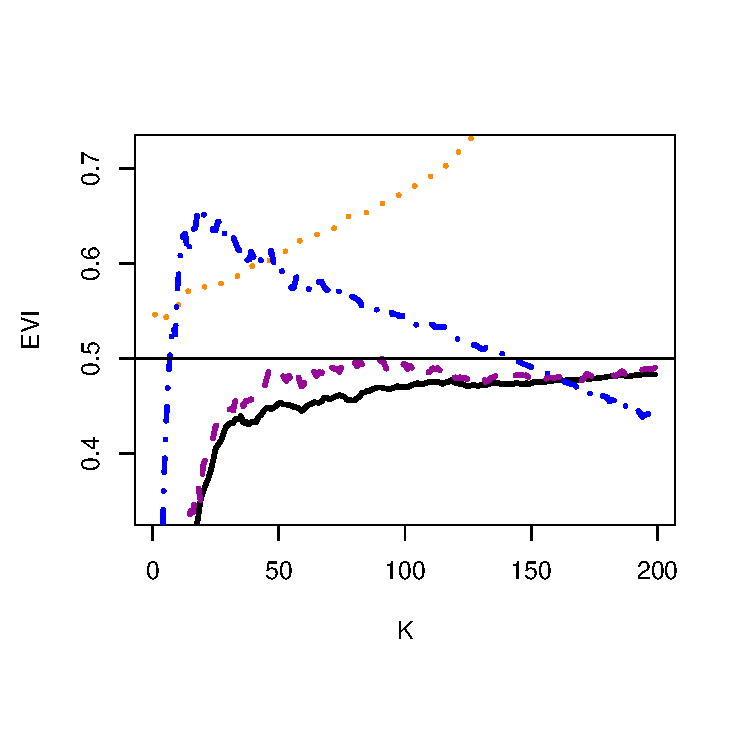
\includegraphics[width=0.45\textwidth]{burr05GPD_evi.pdf} 
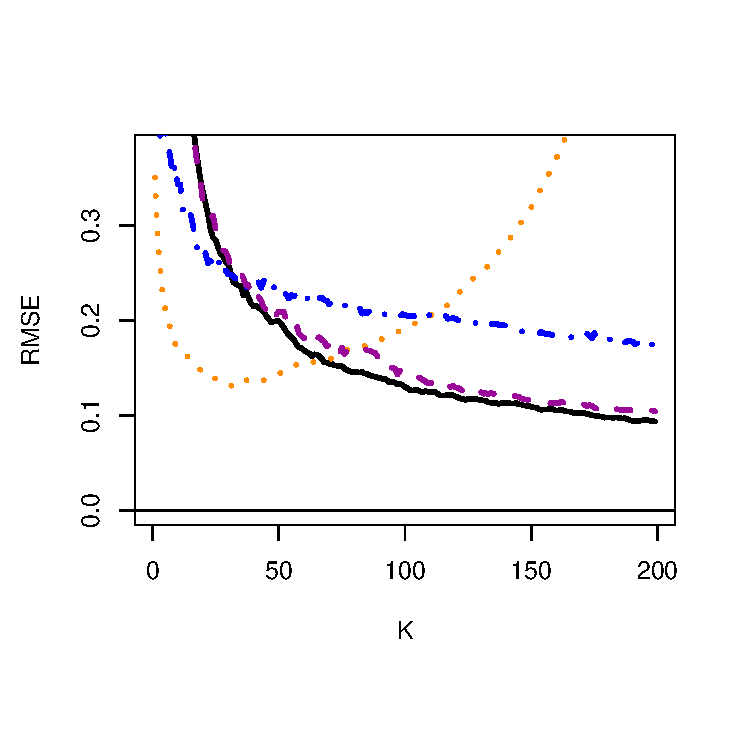
\includegraphics[width=0.45\textwidth]{burr05GPD_rmse.pdf} \\
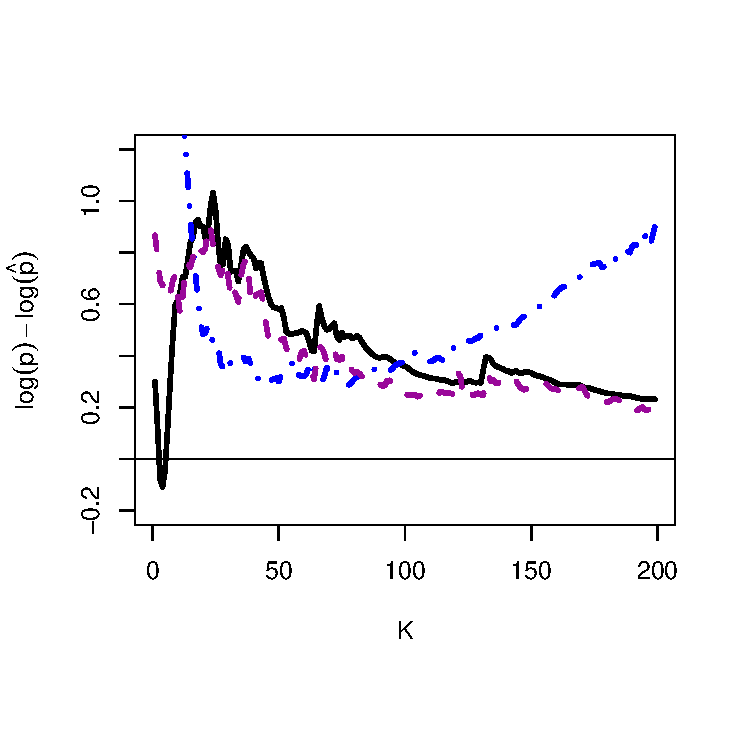
\includegraphics[width=0.45\textwidth]{burr05GPD_tail.pdf}
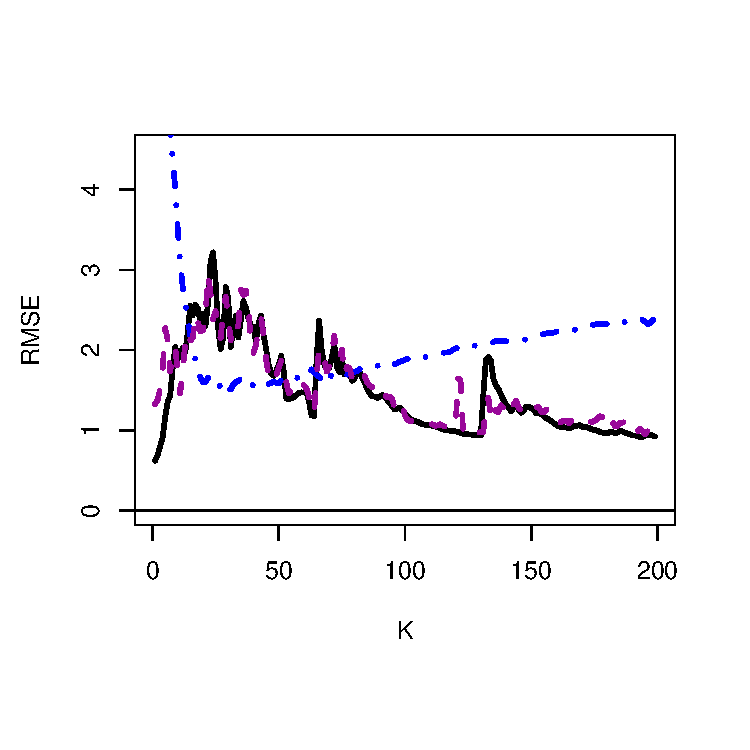
\includegraphics[width=0.45\textwidth]{burr05GPD_tail_rmse.pdf}  
 \caption{ Burr distribution with $\xi=0.5$ and $\rho=-0.5$. Estimation of $\xi$ (top) and tail probability (bottom) using minimum variance principle, bias (left), RMSE (right): GPD-ML (full line), $Ep$ (dash-dotted), $E\bar{p}$ (dashed) and ridge regression estimator (dotted). }
\end{figure}
 \begin{figure}[!ht]
  \centering
  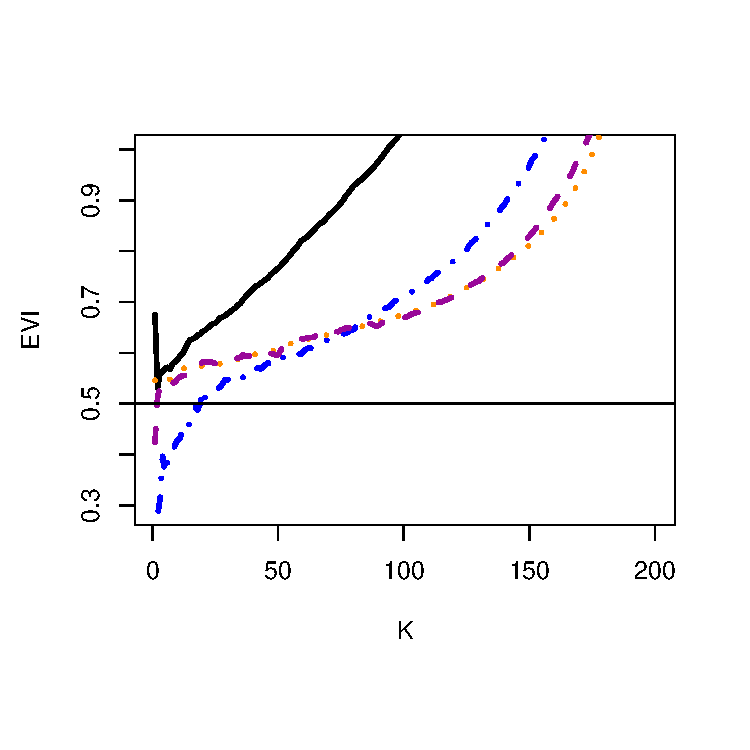
\includegraphics[width=0.45\textwidth]{burr05Pareto_evi.pdf} 
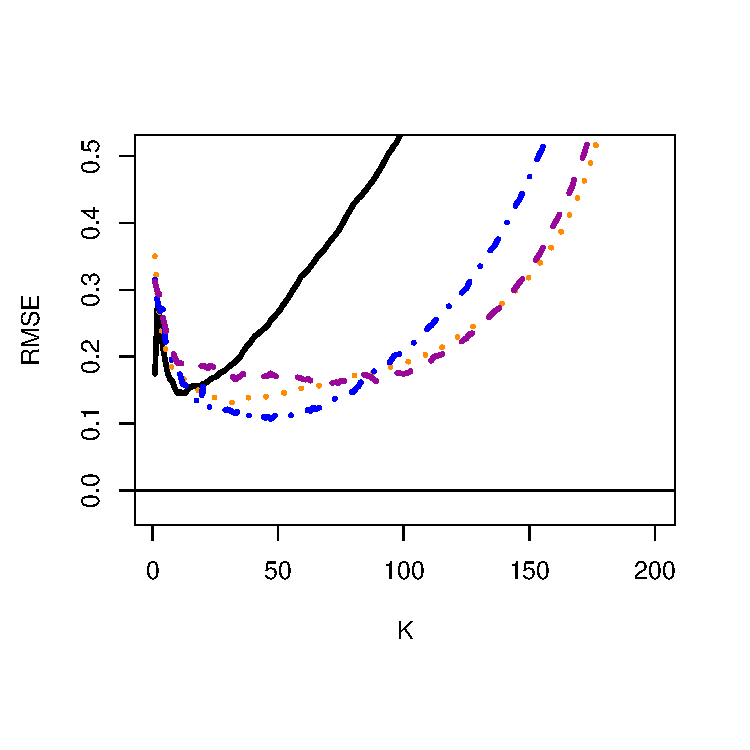
\includegraphics[width=0.45\textwidth]{burr05Pareto_rmse.pdf} \\
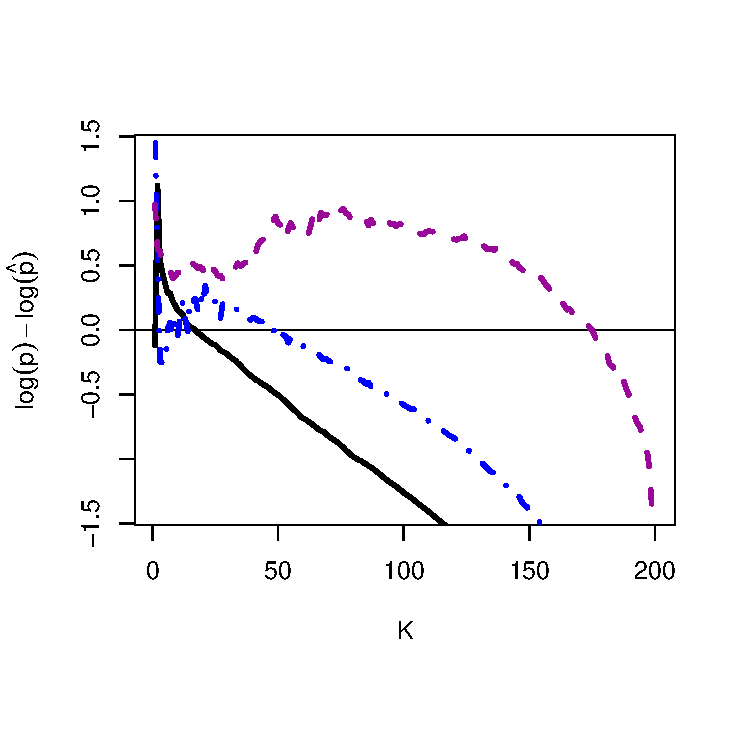
\includegraphics[width=0.45\textwidth]{burr05Pareto_tail.pdf}
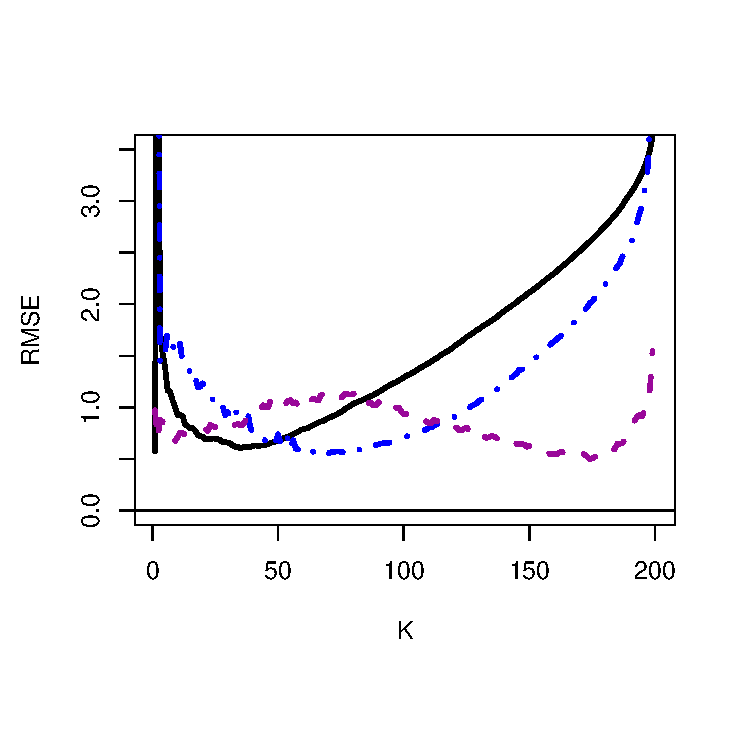
\includegraphics[width=0.45\textwidth]{burr05Pareto_tail_rmse.pdf} 
\caption{Burr distribution with $\xi=0.5$ and $\rho=-0.5$. Estimation of $\xi$ (top) and tail probability (bottom) using minimum variance principle, bias (left), RMSE (right): Pareto-ML (full line), $Ep^+$ (dash-dotted), $E\bar{p}^+$ (dashed) and corrected Hill estimator (dotted).}
  \end{figure}
  
  \begin{figure}[!ht]
  \centering
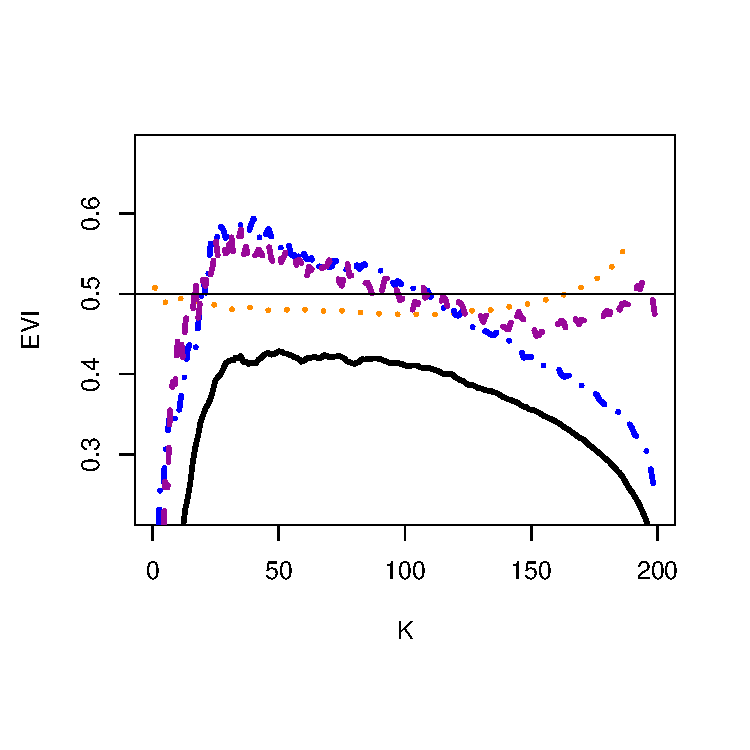
\includegraphics[width=0.45\textwidth]{frechetGPD_evi.pdf} 
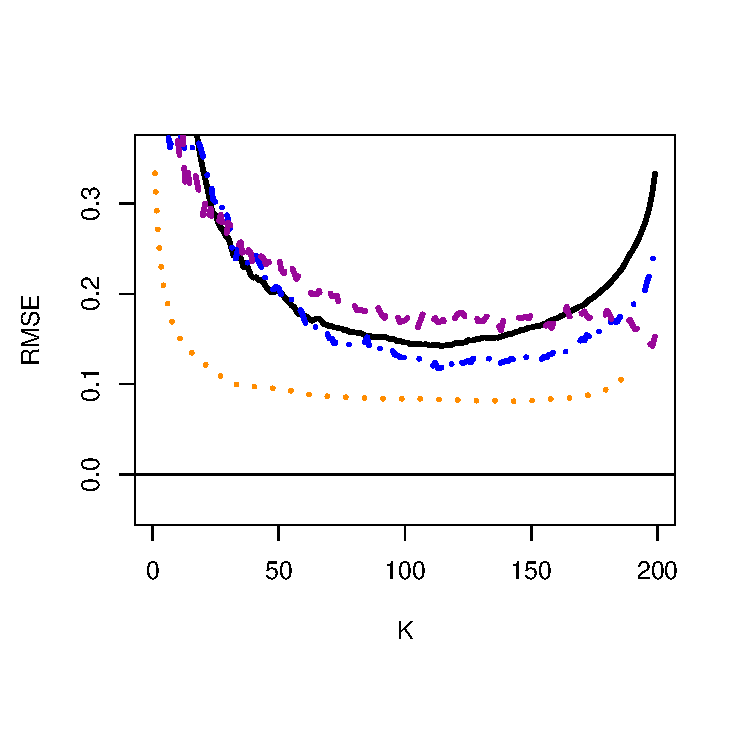
\includegraphics[width=0.45\textwidth]{frechetGPD_rmse.pdf} \\
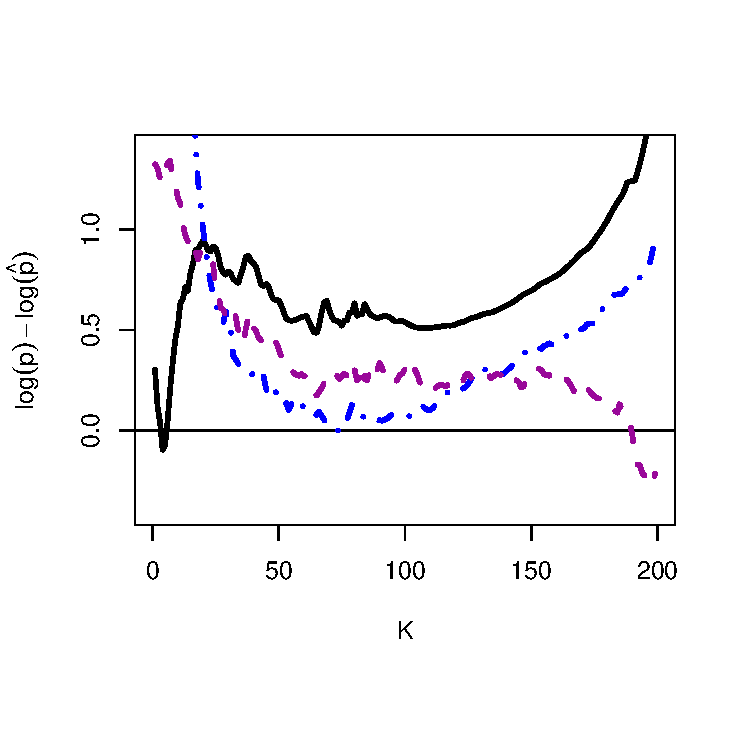
\includegraphics[width=0.45\textwidth]{frechetGPD_tail.pdf}
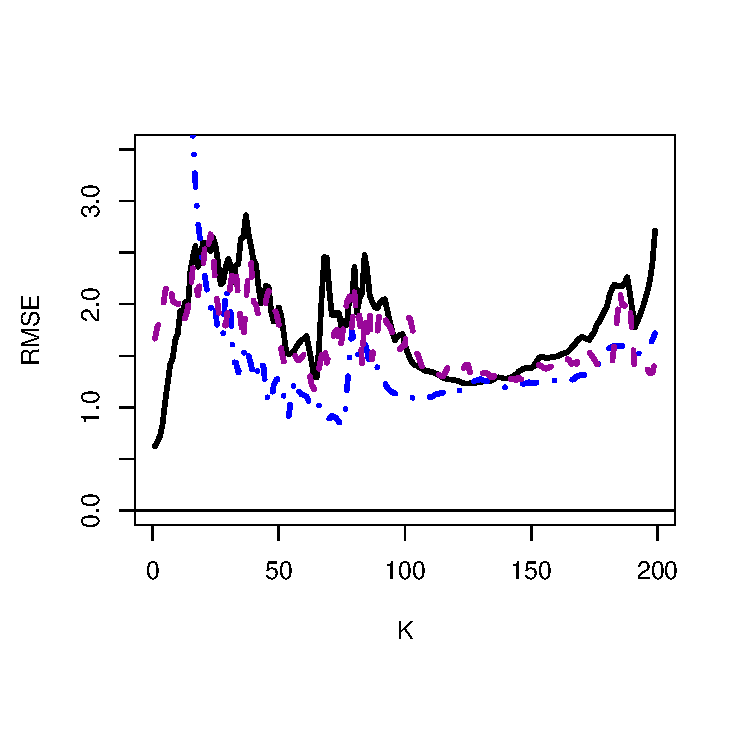
\includegraphics[width=0.45\textwidth]{frechetGPD_tail_rmse.pdf}  
 \caption{ Fr\'echet distribution with $\xi=0.5$. Estimation of $\xi$ (top) and tail probability (bottom), bias (left), RMSE (right): GPD-ML (full line), $Ep$ with $\rho=-2$ (dash-dotted), $E\bar{p}$ with $(k_*,m)=(190,150)$ (dashed), and ridge regression estimator (dotted). }
\end{figure}
 \begin{figure}[!ht]
  \centering
  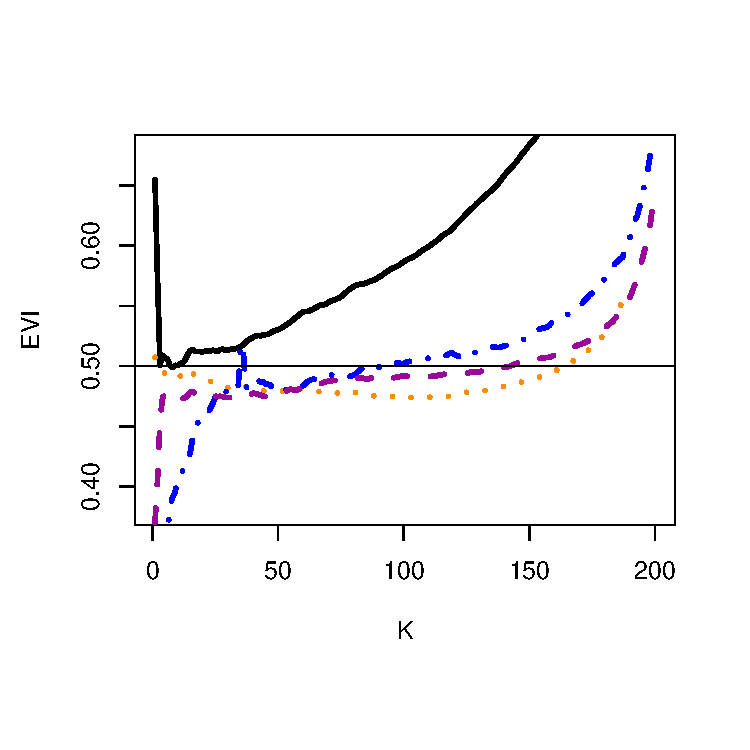
\includegraphics[width=0.45\textwidth]{frechetPareto_evi.pdf} 
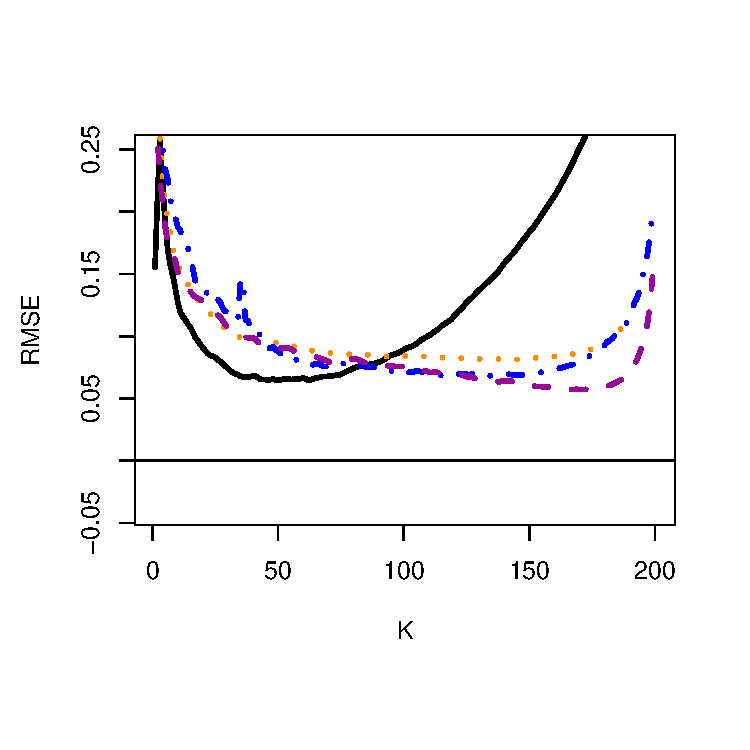
\includegraphics[width=0.45\textwidth]{frechetPareto_rmse.pdf} \\
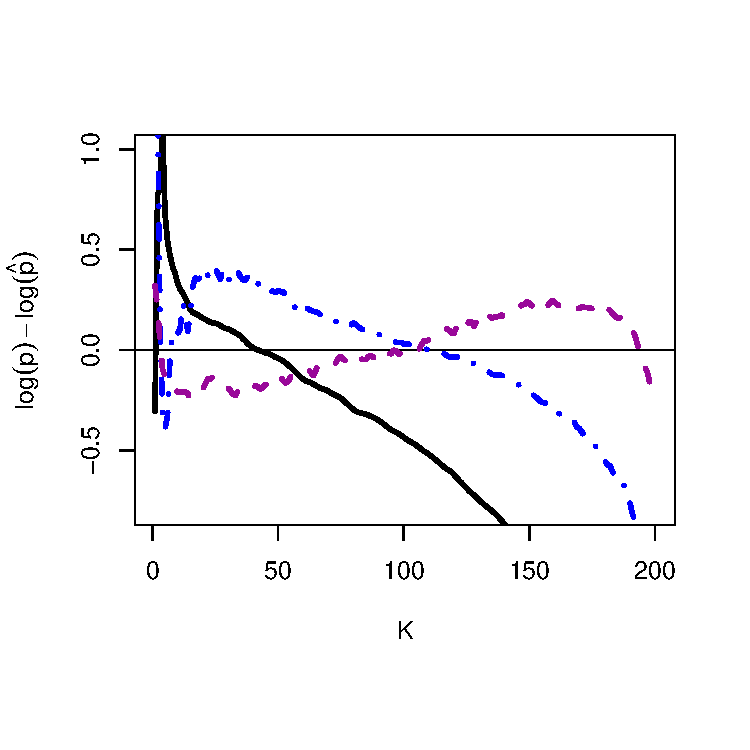
\includegraphics[width=0.45\textwidth]{frechetPareto_tail.pdf}
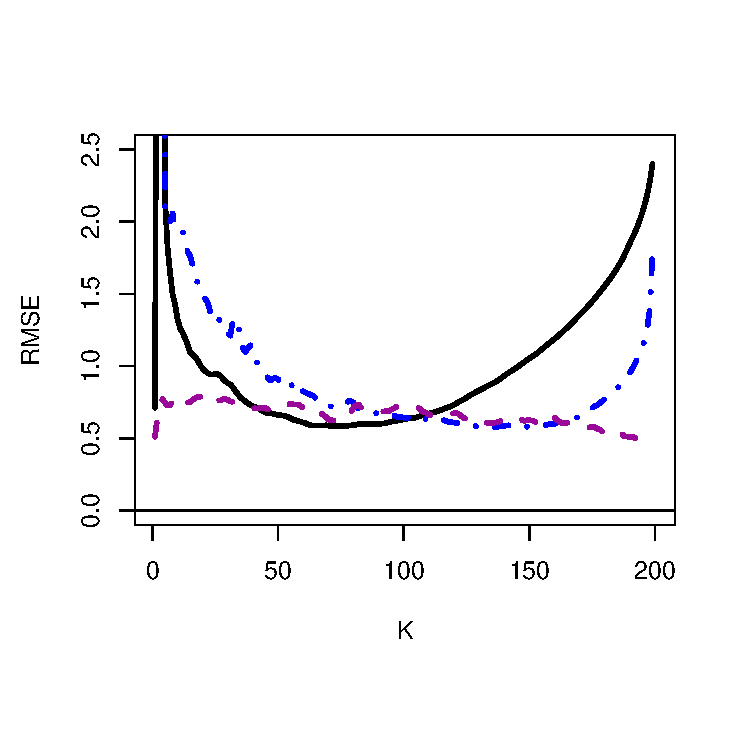
\includegraphics[width=0.45\textwidth]{frechetPareto_tail_rmse.pdf} 
\caption{Fr\'echet distribution with $\xi=0.5$. Estimation of $\xi$ (top) and tail probability (bottom) using minimum variance principle, bias (left), RMSE (right): Pareto-ML  (full line), $Ep^+$ (dash-dotted), $E\bar{p}^+$ (dashed) and corrected Hill estimator (dotted).}
  \end{figure}
  \begin{figure}[!ht]
  \centering
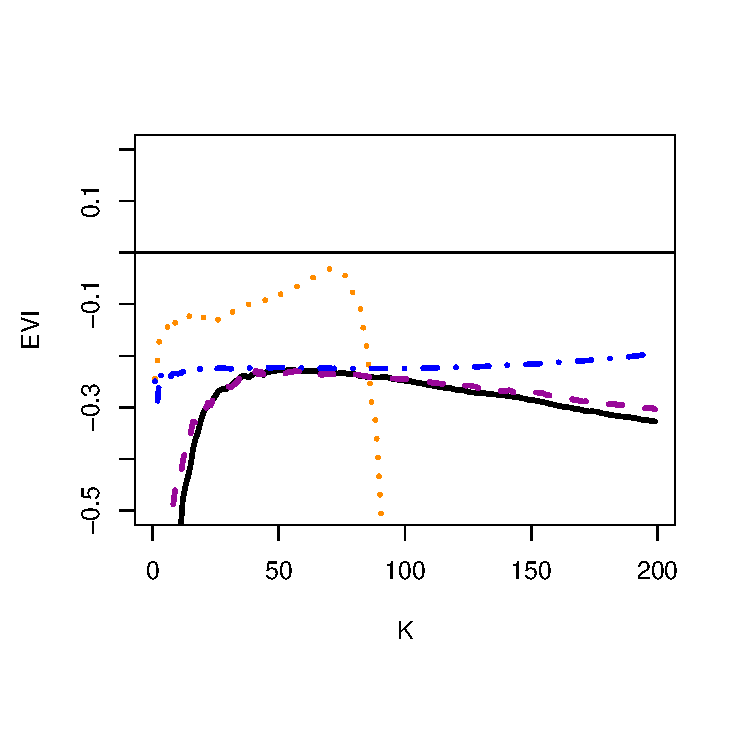
\includegraphics[width=0.45\textwidth]{std_normalGPD_evi.pdf} 
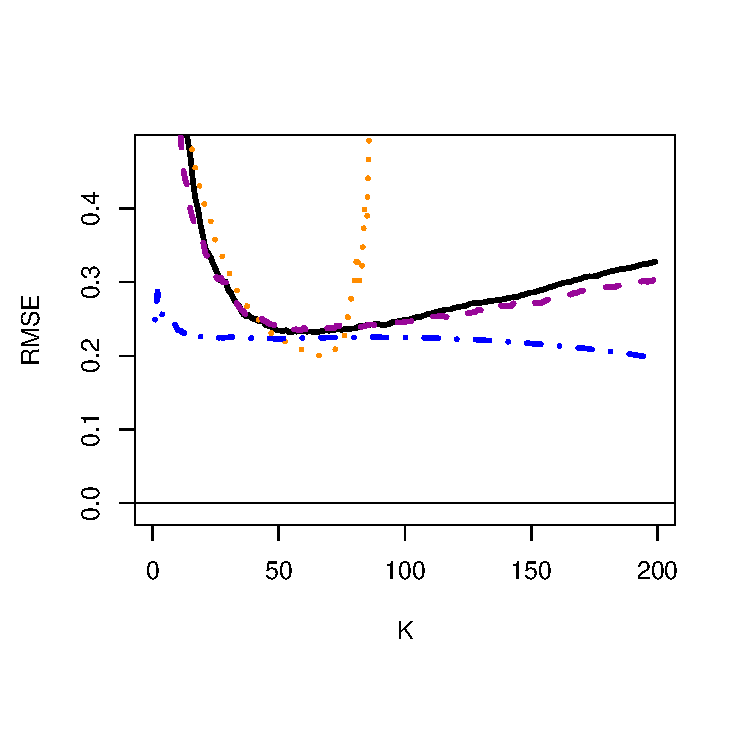
\includegraphics[width=0.45\textwidth]{std_normalGPD_rmse.pdf} \\
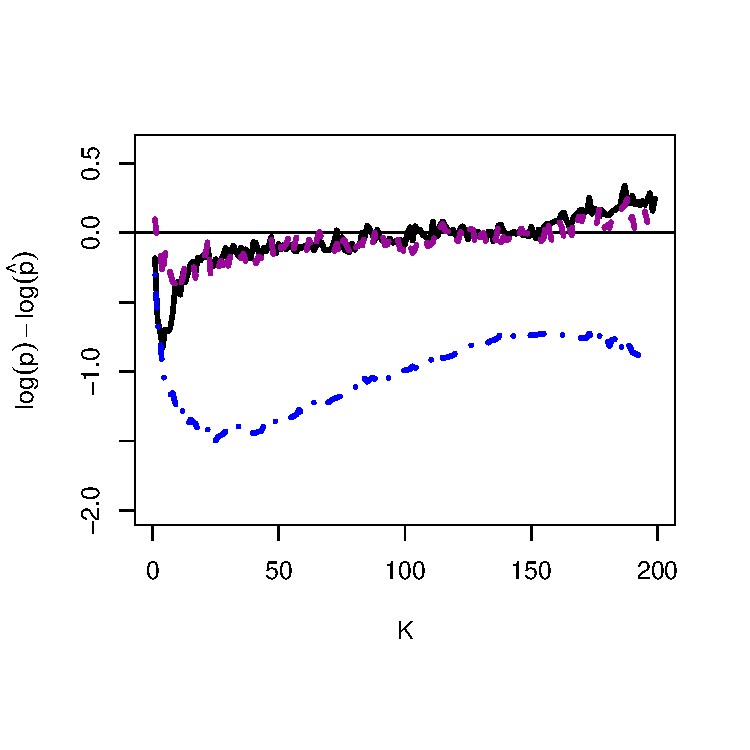
\includegraphics[width=0.45\textwidth]{std_normalGPD_tail.pdf}
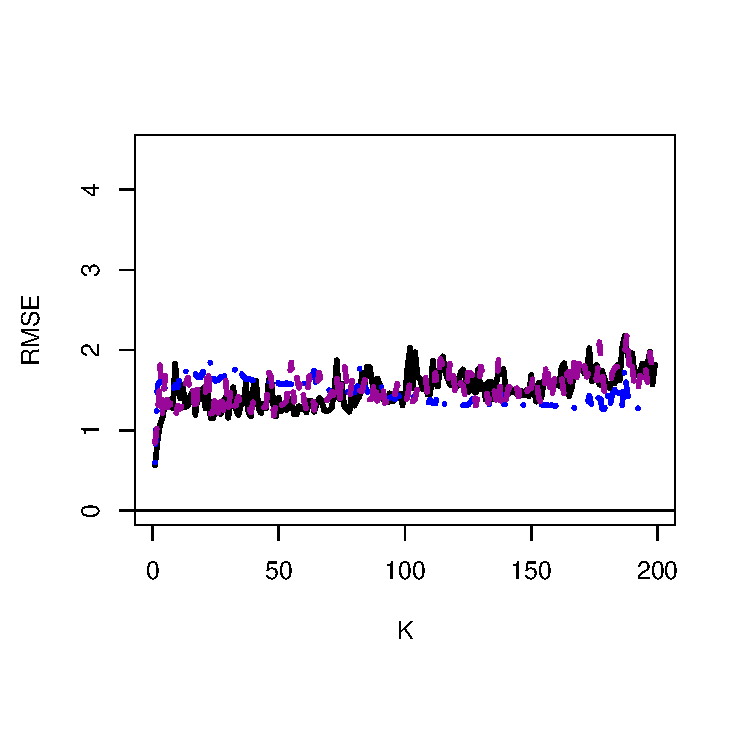
\includegraphics[width=0.45\textwidth]{std_normalGPD_tail_rmse.pdf}  
 \caption{ Standard normal distribution ($\xi=0$ and $\tilde\rho=0$). Estimation of $\xi$ (top) and tail probability (bottom) using minimum variance principle, bias (left), RMSE (right): GPD-ML (full line), $Ep$ (dash-dotted), $E\bar{p}$ (dashed) and ridge regression estimator (dotted).}
\end{figure}

 \begin{figure}[!ht]
  \centering
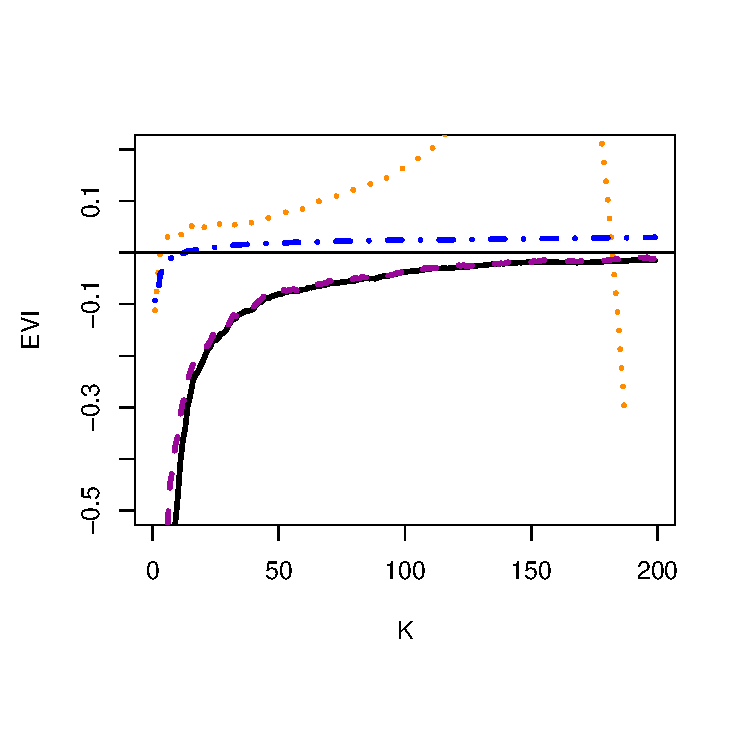
\includegraphics[width=0.45\textwidth]{exponentialGPD_evi.pdf} 
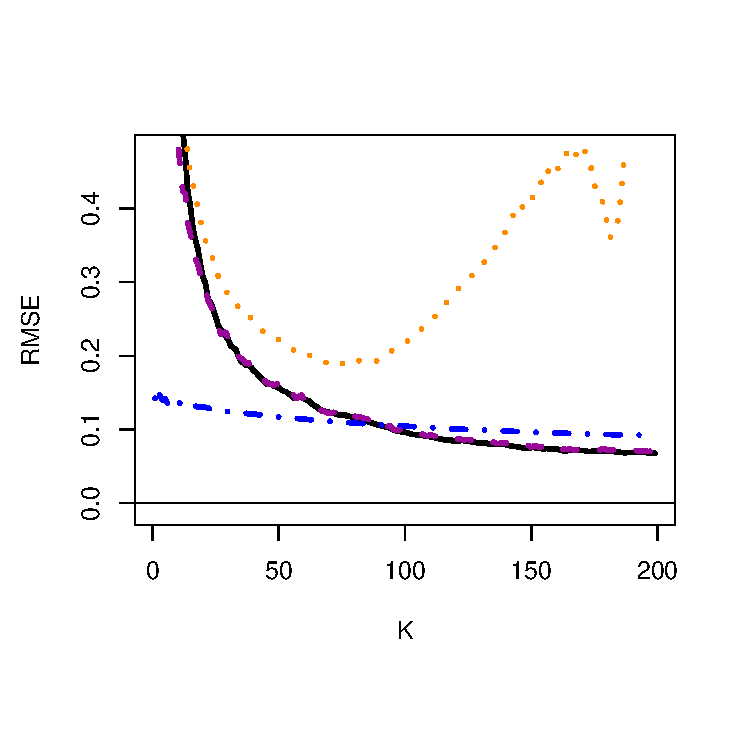
\includegraphics[width=0.45\textwidth]{exponentialGPD_rmse.pdf} \\
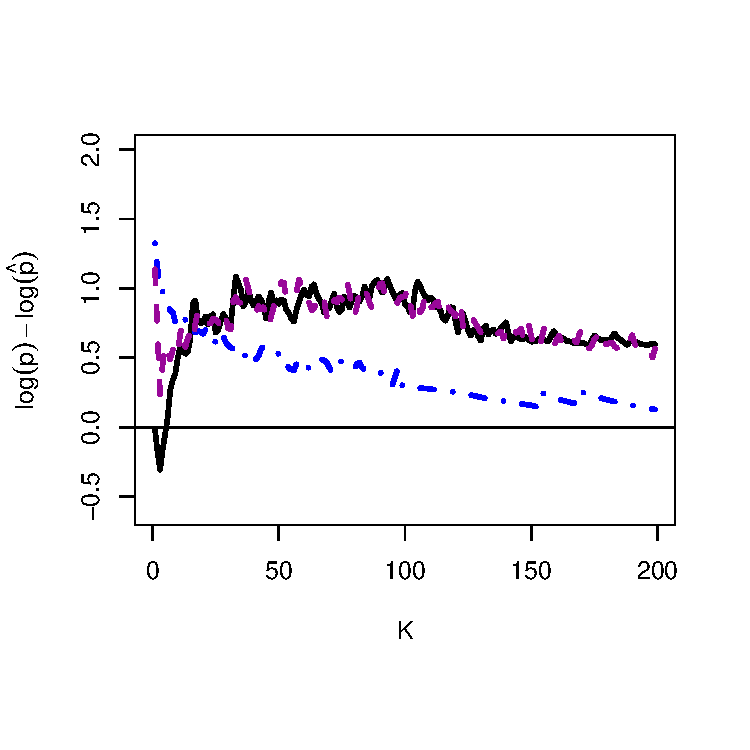
\includegraphics[width=0.45\textwidth]{exponentialGPD_tail.pdf}
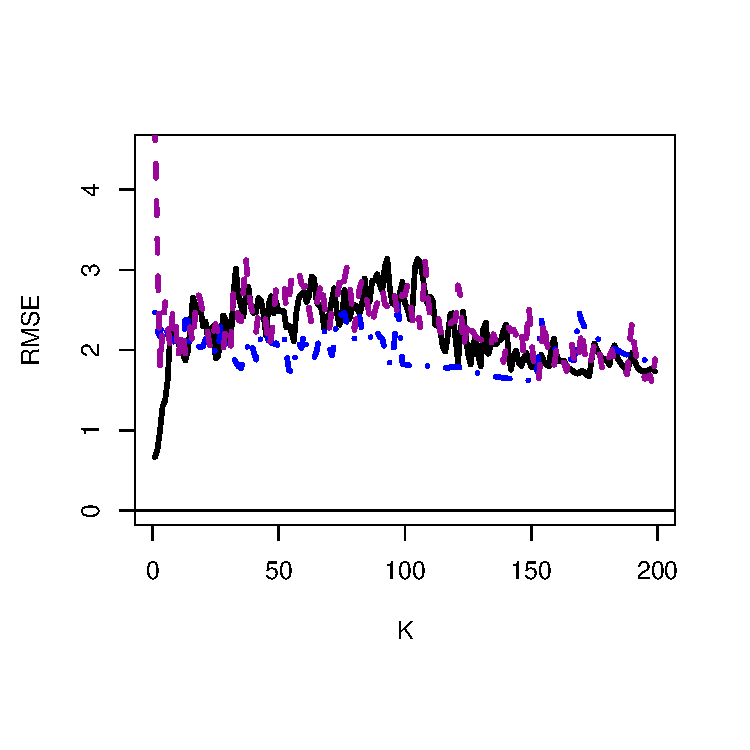
\includegraphics[width=0.45\textwidth]{exponentialGPD_tail_rmse.pdf}  
 \caption{ The exponential distribution ($\xi=0$ and $\tilde\rho=0$). Estimation of $\xi$ (top) and tail probability (bottom) using minimum variance principle, bias (left), RMSE (right): GPD-ML (full line),  $Ep$ (dash-dotted), $E\bar{p}$ (dashed) and ridge regression estimator (dotted).}
\end{figure}

 

 \begin{figure}[!ht]
  \centering
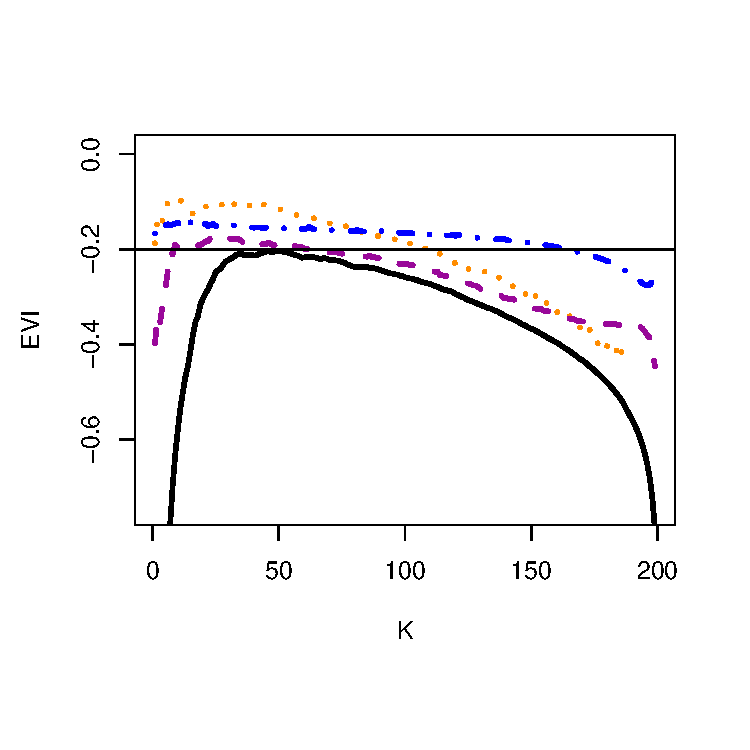
\includegraphics[width=0.45\textwidth]{model3GPD_evi.pdf} 
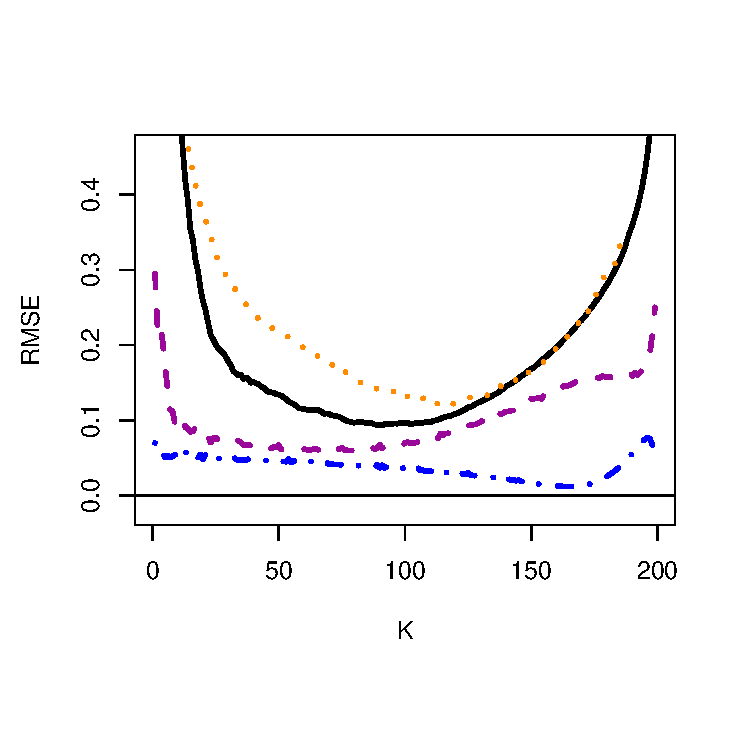
\includegraphics[width=0.45\textwidth]{model3GPD_rmse.pdf} \\
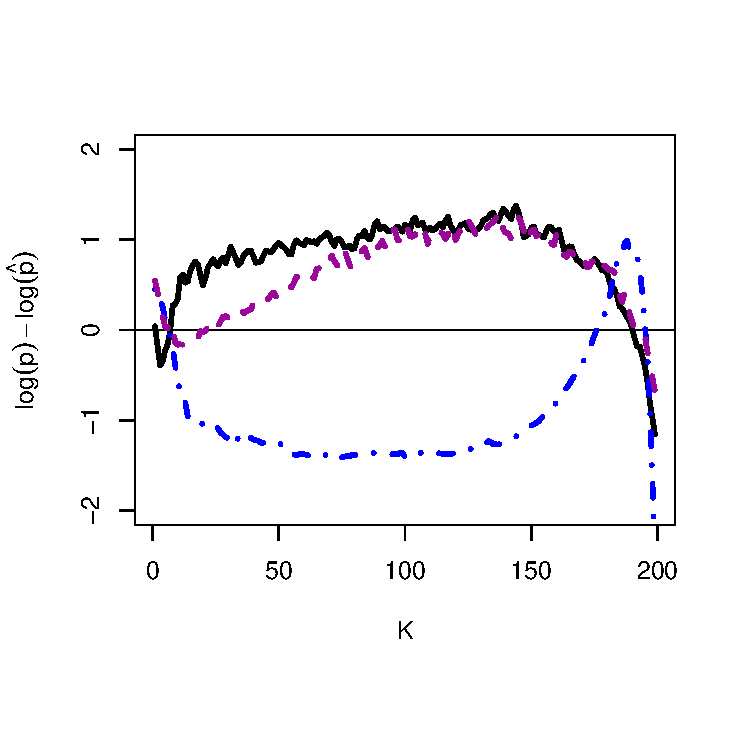
\includegraphics[width=0.45\textwidth]{model3GPD_tail.pdf}
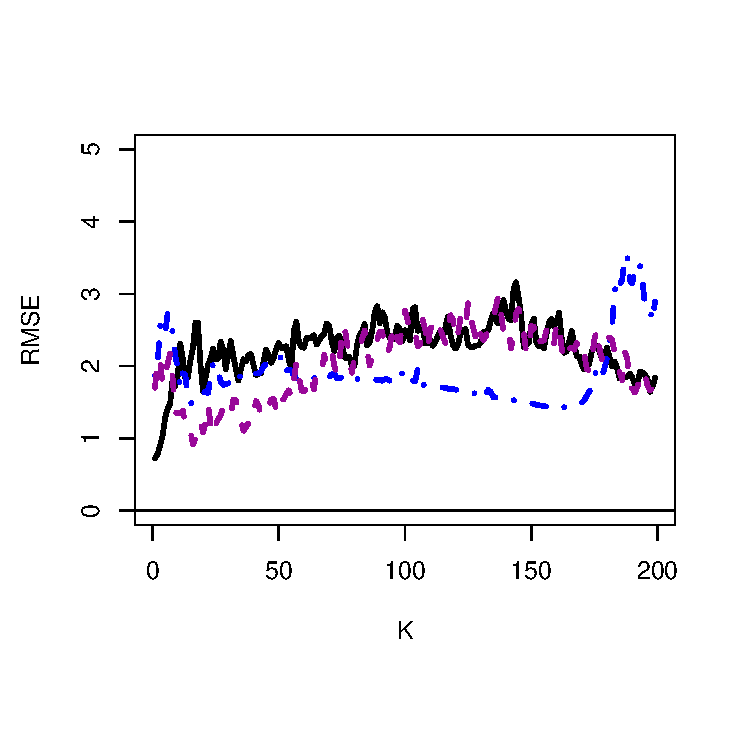
\includegraphics[width=0.45\textwidth]{model3GPD_tail_rmse.pdf}  
 \caption{ Reversed Burr distribution ($\xi=-0.2$ and $\tilde\rho=-1$). Estimation of $\xi$ (top) and tail probability (bottom) using minimum variance principle, bias (left), RMSE (right): GPD-ML (full line),  $Ep$ (dash-dotted), $E\bar{p}$ (dashed) and ridge regression estimator (dotted).}
\end{figure}

\begin{figure}[!ht]
  \centering
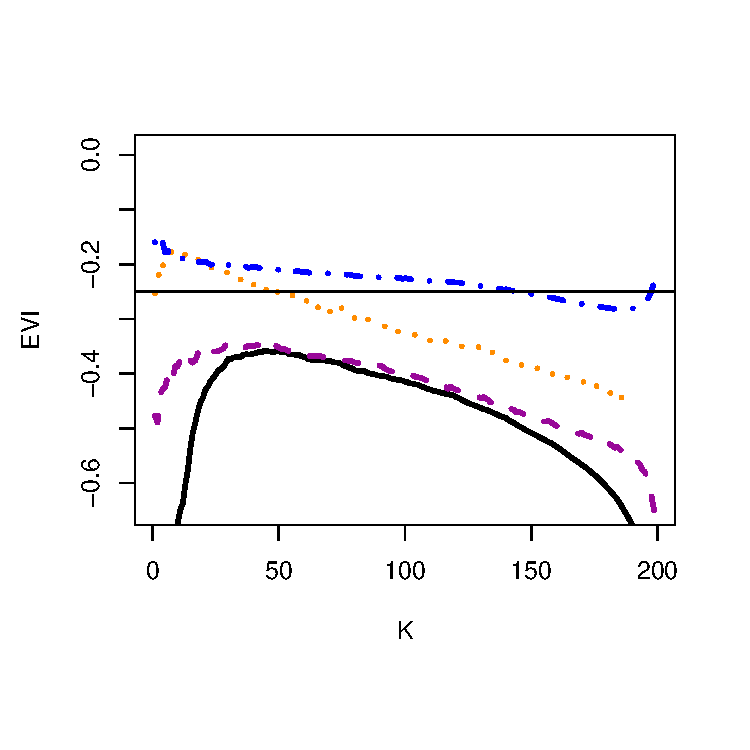
\includegraphics[width=0.45\textwidth]{weibullGPD_evi.pdf} 
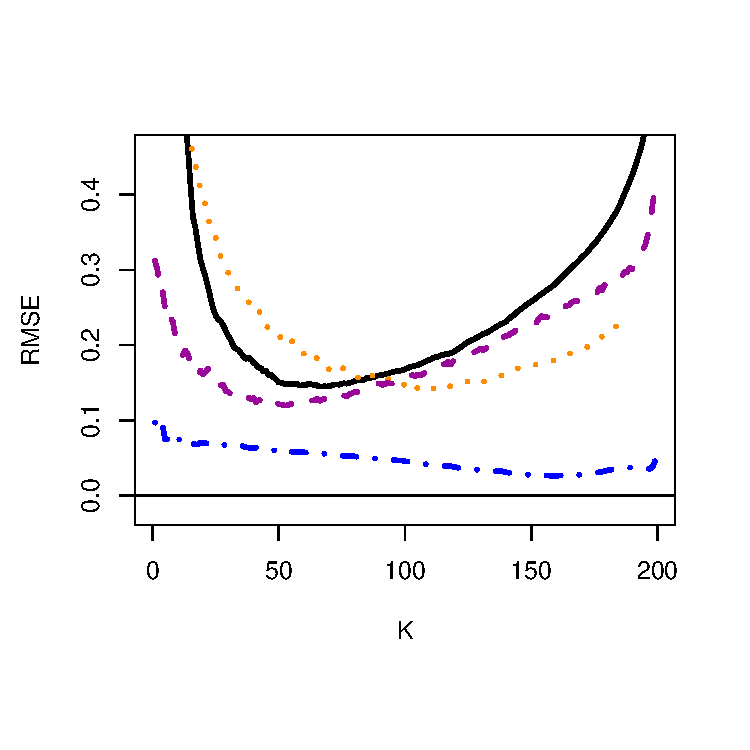
\includegraphics[width=0.45\textwidth]{weibullGPD_rmse.pdf} \\
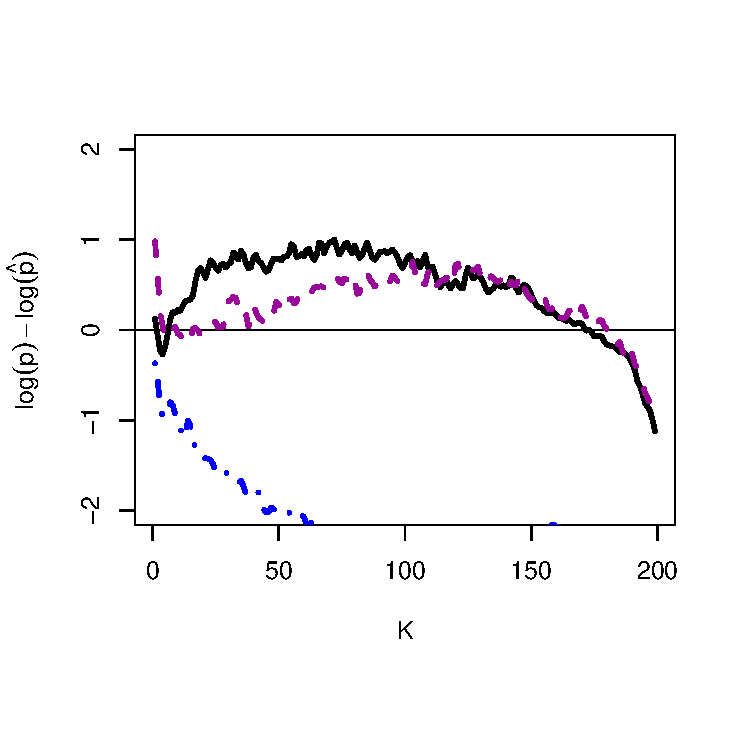
\includegraphics[width=0.45\textwidth]{weibullGPD_tail.pdf}
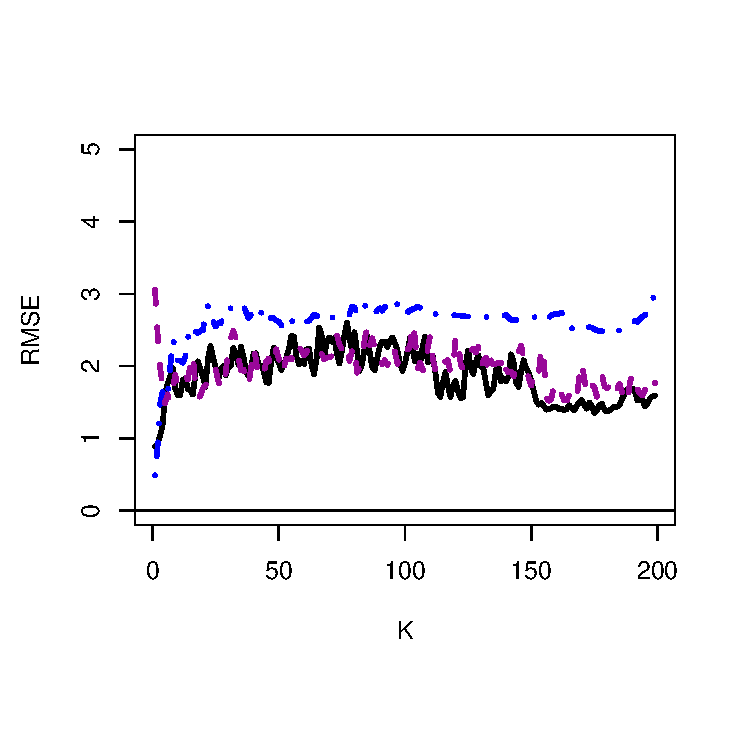
\includegraphics[width=0.45\textwidth]{weibullGPD_tail_rmse.pdf}  
 \caption{Extreme value Weibull distribution ($\xi=-0.25$ and $\tilde\rho=-1$). Estimation of $\xi$ (top) and tail probability (bottom) using minimum variance principle, bias (left), RMSE (right): GPD-ML (full line), $Ep$ (dash-dotted), $E\bar{p}$ (dashed) and ridge regression estimator (dotted).}
\end{figure}

\begin{figure}[!ht]
  \centering
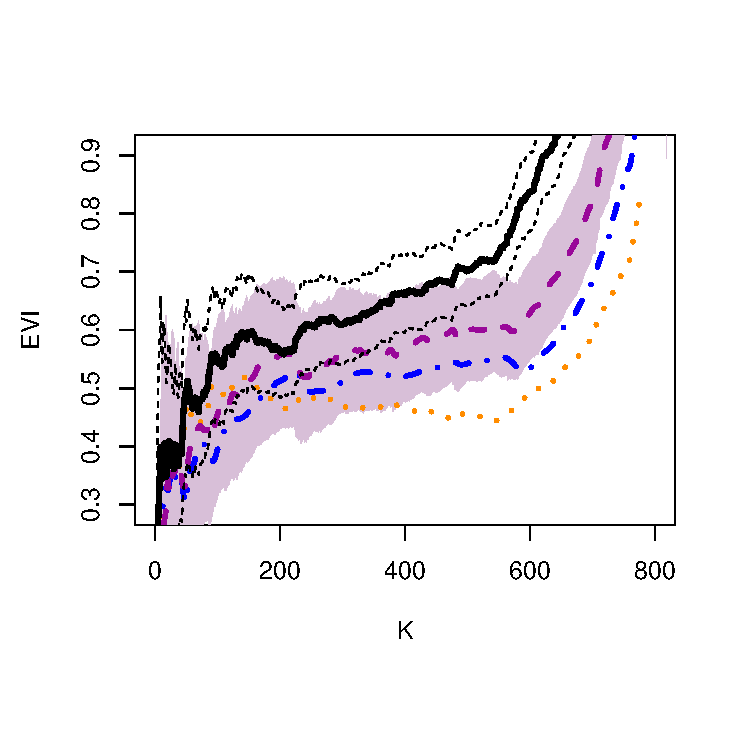
\includegraphics[width=0.45\textwidth]{ultimates_evi.pdf} 
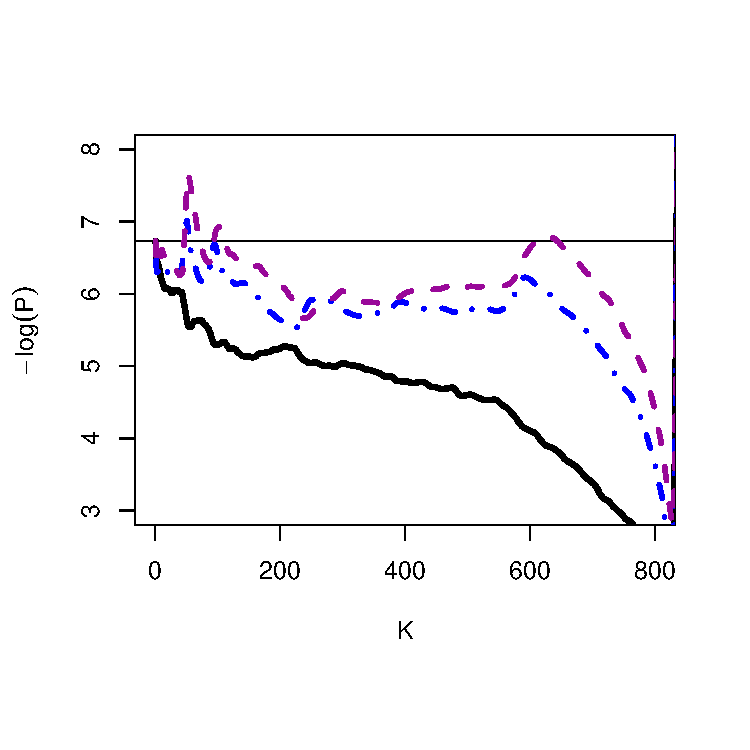
\includegraphics[width=0.45\textwidth]{ultimates_tail.pdf} 
\\
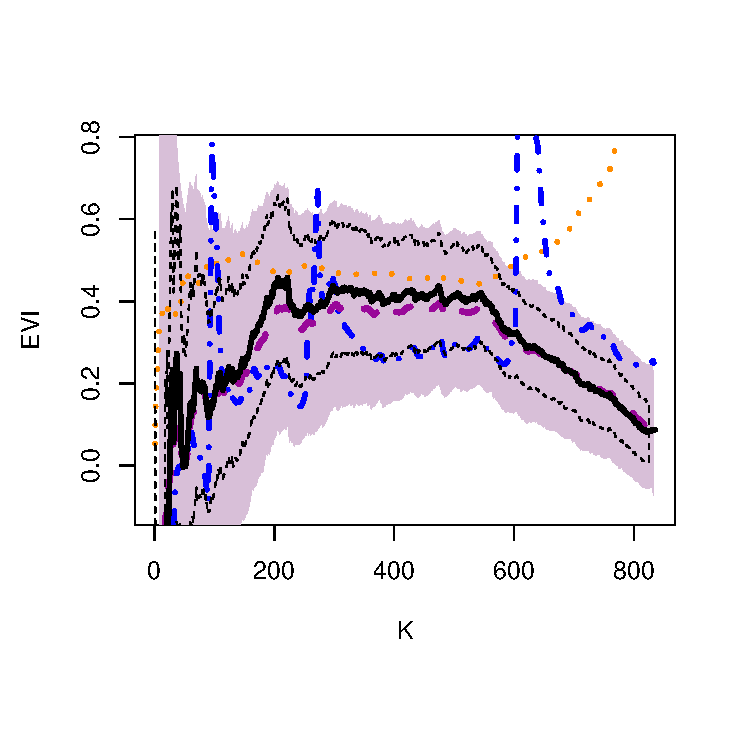
\includegraphics[width=0.45\textwidth]{ultimates_gp_evi.pdf} 
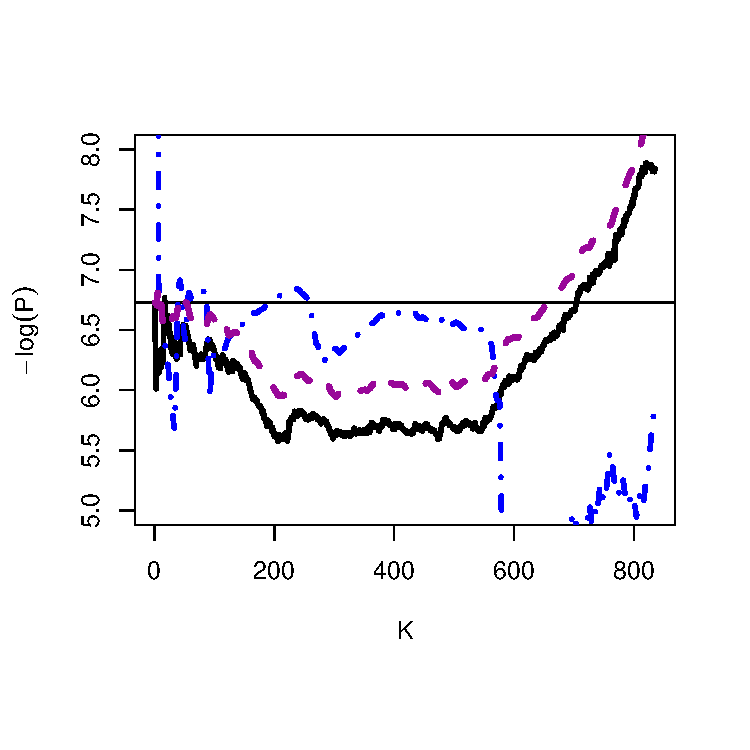
\includegraphics[width=0.45\textwidth]{ultimates_gp_tail.pdf} 
%\includegraphics[width=0.45\textwidth]{ultimates_GoF.pdf}
  \caption{Ultimates of Belgian car insurance claims: estimation of $\xi$ with asymptotic confidence intervals (left), tail probability estimation at maximum observation (right), Pareto-based analysis (top) and GPD-based analysis (bottom): classical ML estimation (full line with dotted confidence intervals), $Ep$ (dashed with shaded confidence intervals) and $E\bar{p}$ (dash-dotted). CH (top left)  and ridge regression (bottom left) estimators are indicated by dotted lines.}
\end{figure} 

\begin{figure}[!ht]
  \centering
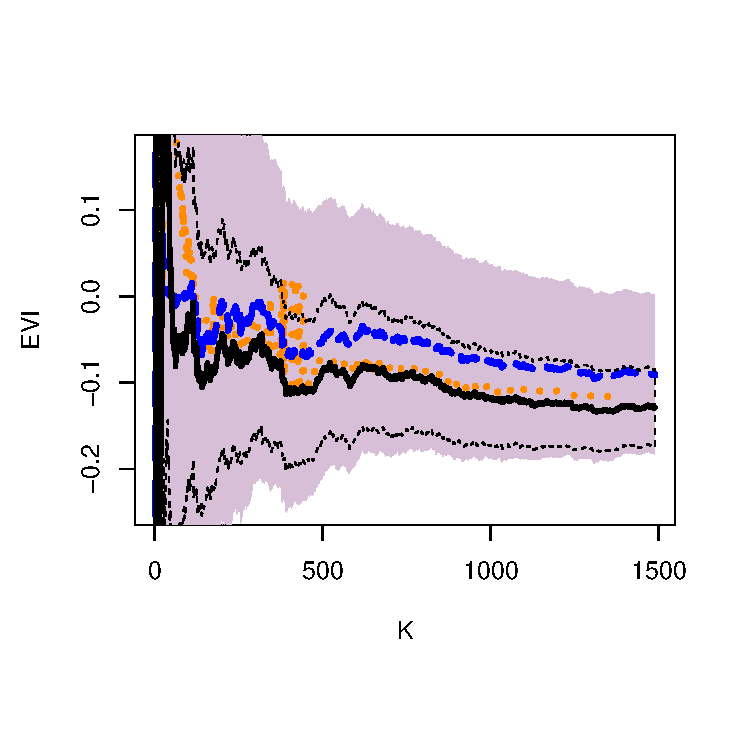
\includegraphics[width=0.45\textwidth]{lifetime_evi_with_GPD_conf.pdf} 
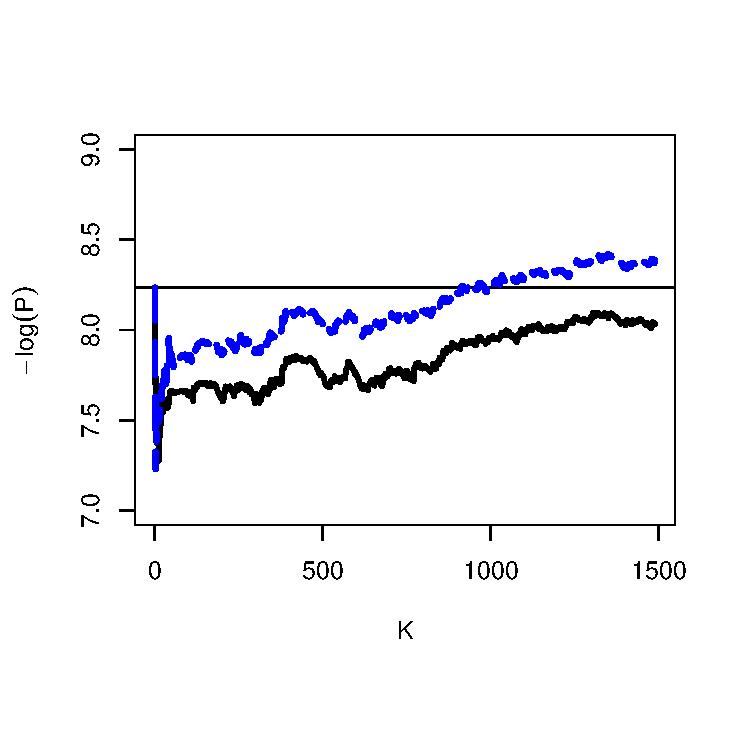
\includegraphics[width=0.45\textwidth]{lifetime_prob.pdf} 
  \caption{Lifetime data from the Netherlands, female persons who died in 1986. Left: estimation of $\xi$ with asymptotic confidence intervals for classical ML estimation (full line with dotted confidence intervals), $Ep$ (dashed with shaded confidence intervals, $\tilde\rho=-0.5$) and ridge regression (dotted). Right: tail probability estimation at maximum observation for classical ML estimation (full line) and  $Ep$ (dashed). }
\end{figure} 
 


\end{document}




\subsection{Theoretical background}

As mentioned in section~\ref{Sec1}, in principle, the difficulties raised by the existence of factual items can be tackle by either:
\begin{enumerate}
\item[a)] ignoring the issue and excluding all the possible `problematic' items from XYZ compilation;
\item[b)] allocating fixed weights, assuming that factual items are to be treated in the same way as all other items (this is the fixed weights approach);
\item[c)] allocating variable/changing weights, according to the consumption pattern found in the base year (this is the variable weights approach).
\end{enumerate}

Table~\ref{Tab1} summarises the main advantages and disadvantages of the three considered approaches.

\vspace*{5mm}
\begin{table}[h]
\centering
\begin{tabular}{|c|c|c|}
\hline
\textbf{Approach} & \textbf{Advantages} & \textbf{Disadvantages}\\
\hline
Ignore... & Simplicity & Overlooking...\\
Fixed-weight & Theoretical consistency & Choice of imputation... \\
Variable-weight & Minimisation... & Theoretical inconsistency\\
\hline
\end{tabular}
\caption{Advantages and disadvantages of different approaches to the treatment of factual items in a XYZ.
\label{Tab1}}
\end{table}
\vspace*{5mm}

Ignoring the `problematic' or more `volatile' items can be seen as a non-solution in the context of an index that wants to reflect changes in consumption prices. If these items have some importance in the XYZ basket, then there is, in principle, no reason for ignoring them.

Figure~\ref{Fig1} compares the carry forward and percentage change indices.\break
Although different in level, they nearly have the same turning points and behaviour in terms of movement.

\vspace*{5mm}
\begin{figure}[h]
\centering
%\includegraphics{rs-fig01.eps}
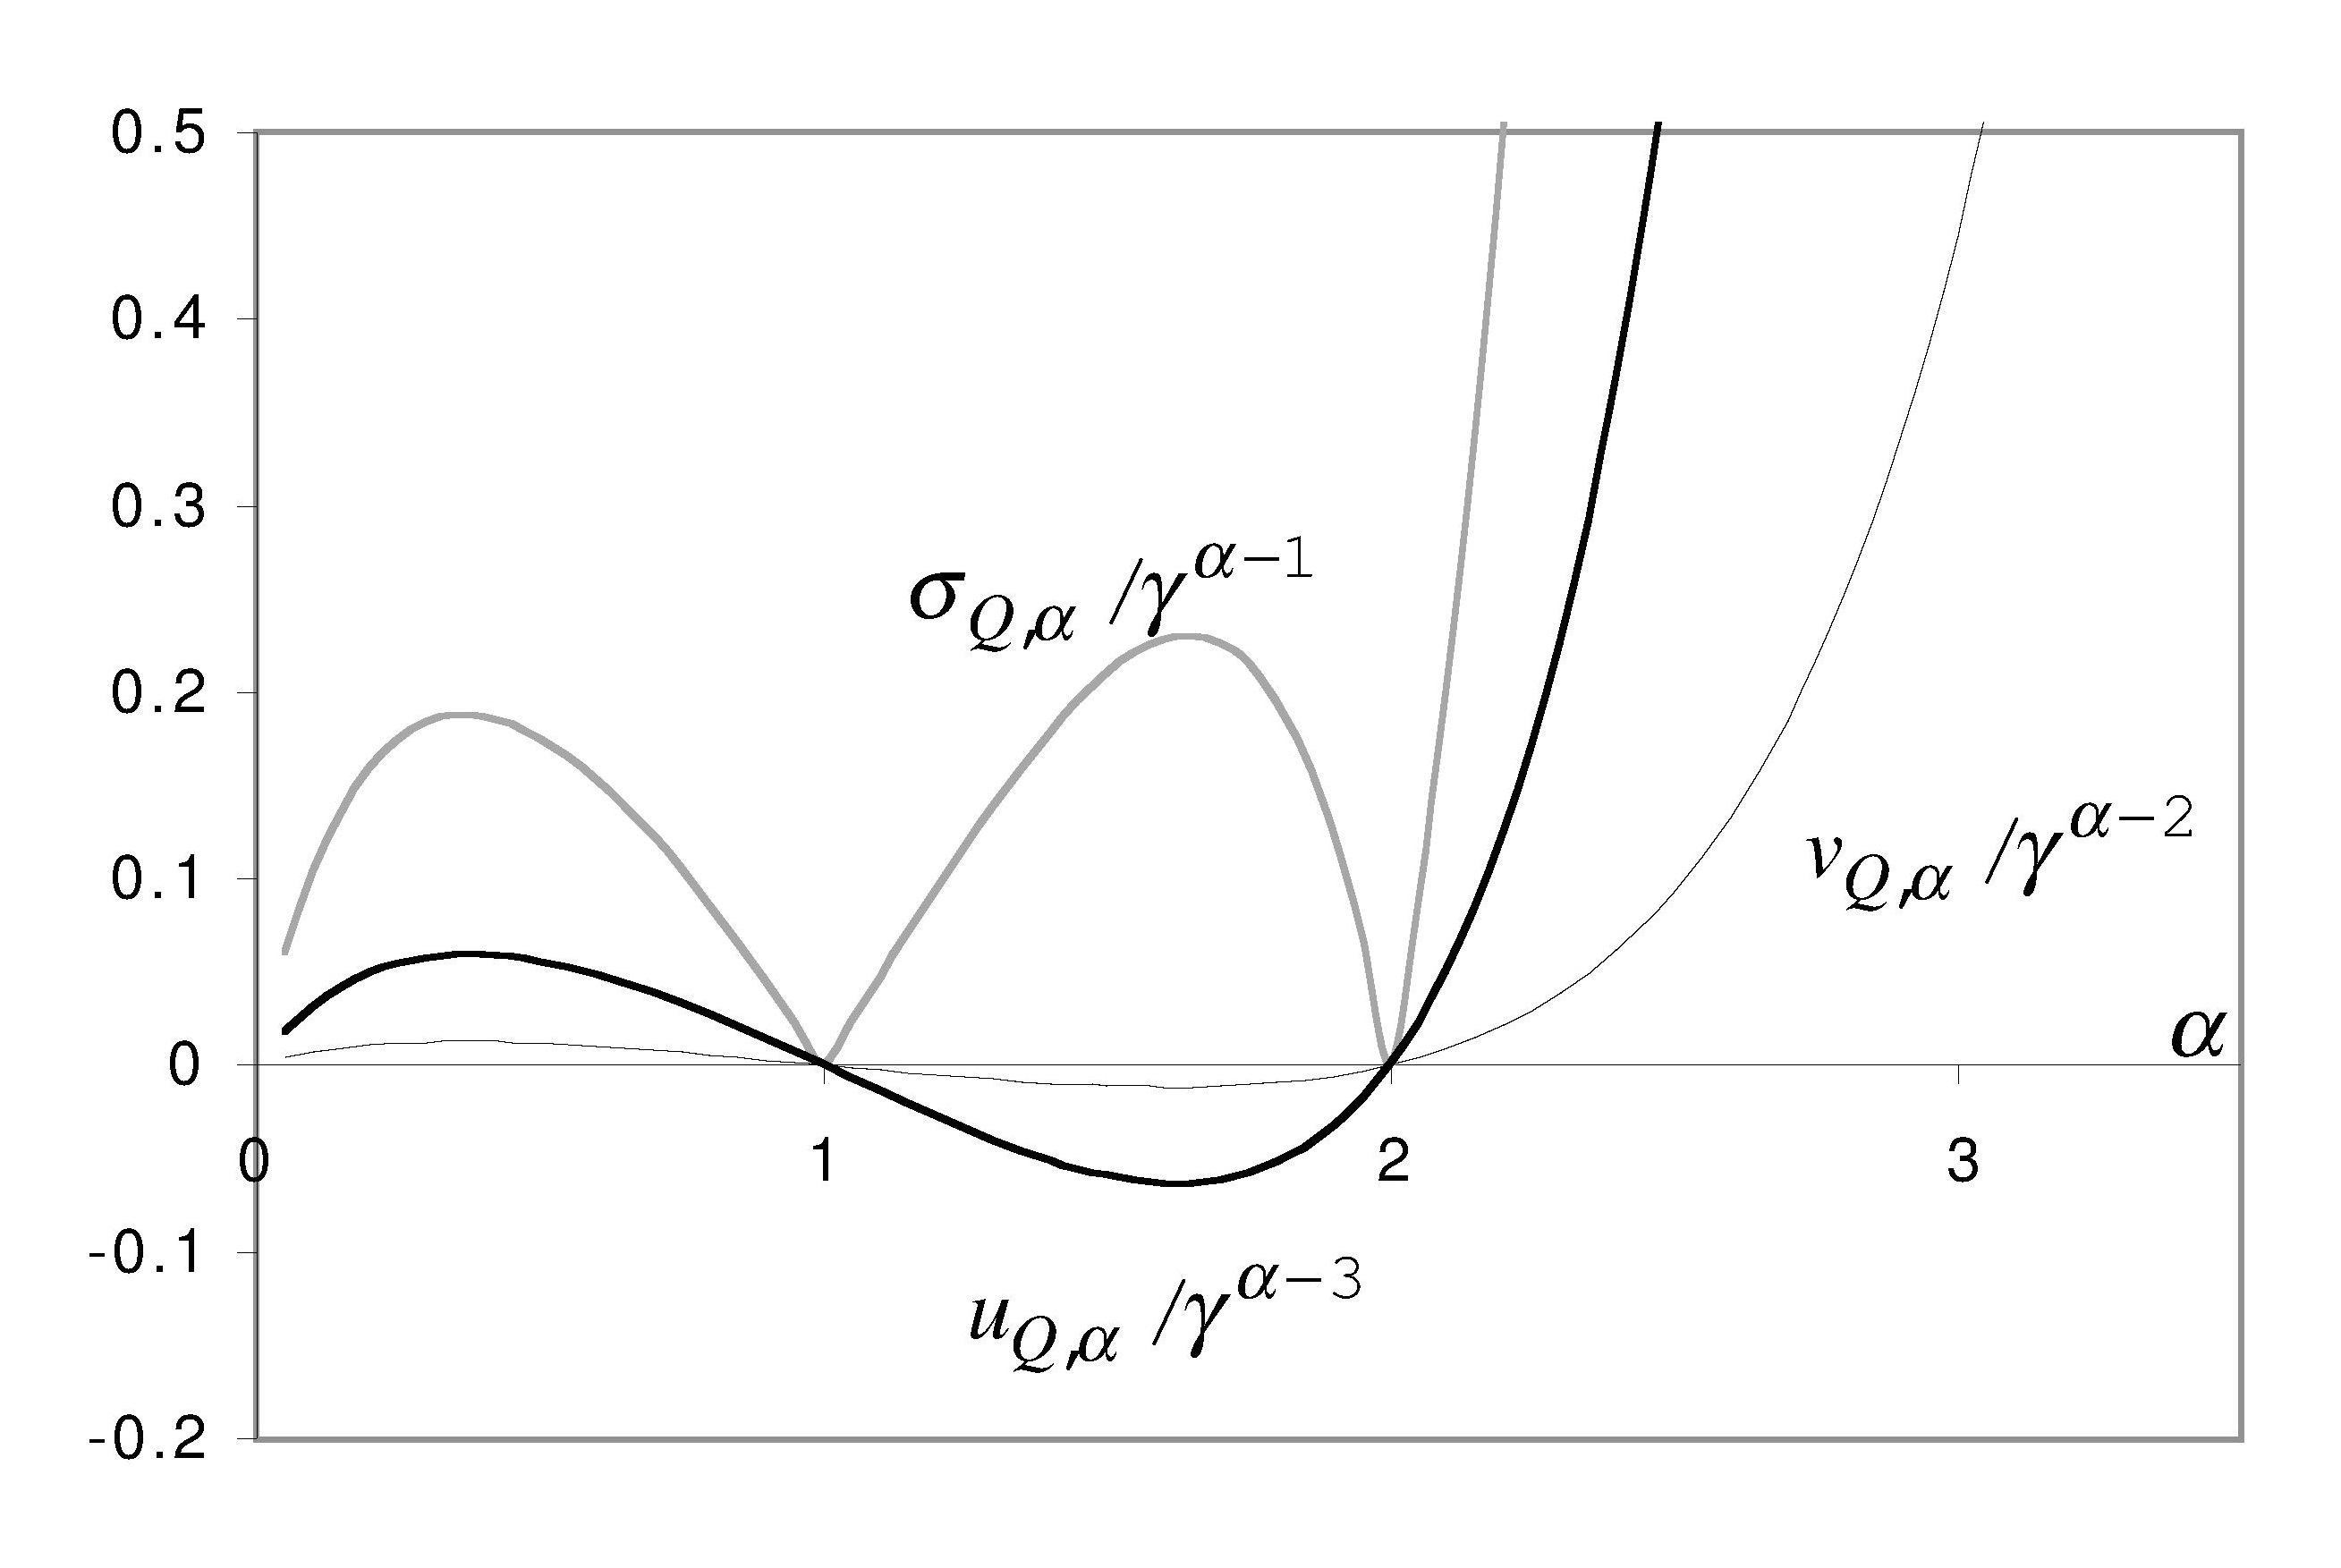
\includegraphics[width=0.7\textwidth]{rs-fig01.png}
\caption{Carry forward and percentage change indices.\hfil\break
Both indices tend to approximate in the months with less prices.
 \label{Fig1}}
\end{figure}
\vspace*{5mm}

\begin{theorem}
\label{Thm1}
Consider aggregation with all the other XYZ components.
\begin{equation}
\label{Eq1}
I_{i;o,m}^{t,m}=\frac{p_{i;t,m}}{p_{i;o,m}}~.
\end{equation}
\end{theorem}

\begin{proof}
This could be the proof of the previous Theorem...
\end{proof}


\subsubsection{This is a subsubsection}

The percentage change index presents a higher volatility than the forward imputation method (\ref{Eq1}), (\ref{Eq2}) and (\ref{Eq3}) (see Theorem~\ref{Thm1} and Lemma~\ref{Lem1}).

\begin{lemma}
\label{Lem1}
Consider aggregation with all the other XYZ components. That is only possible at the class level:
\begin{eqnarray}
\label{Eq2}
 && I_{i;o,m}^{t,m}=\frac{p_{i;t,m}}{p_{i;o,m}}~,~~~~m,n\in\N~;\\[2mm]
\label{Eq3}
 && {}_{s}I_{o,m}^{t,m}=\sum_{i}I_{i;o,m}^{t,m}\,
 \frac{p_{i;t,m}\cdot q_{i;o,m}}{{\displaystyle \sum_{i} p_{i;t,m}\cdot q_{i;o,m}}}~.
\end{eqnarray}
\end{lemma}

No matter which approach is followed, one has to bear in mind that no ``perfect" solution exist...
\\\\
Similar environment for corollary, proposition, ...
%\begin{corollary} \label{Cor1}
% First Corollary...
% \end{corollary}

%\begin{proposition} \label{Pro1}
% First Proposition...
% \end{proposition}

\begin{remark}
\label{Rem1}
First Remark...
\end{remark}

% \begin{note} \label{Not1}
% First Note...
% \end{note}
\noindent
Similar  environment for note, definition, example, ...

% \begin{definition} \label{Def1}
% First Definition...
% \end{definition}

% \begin{example} \label{Exa1}
% First Example...
% \end{example}

\begin{proof}[Proof of Lemma~\ref{Lem1}]
This is the proof of the previous Lemma...
\end{proof}

%-------------------------------------------------------------------------------
% Acknowledgments... Changed in revstat-v2
%-------------------------------------------------------------------------------
\begin{acknowledgments}
This work has been supported by the grant number xyz from Research Institution XX.
We also acknowledge the valuable suggestions from Prof.\ EFG and the referees.
\end{acknowledgments}
%-------------------------------------------------------------------------------
% References...
%-------------------------------------------------------------------------------
\begin{thebibliography}{8}

% --- example of Journal article:
\bibitem{Ab1}
\textsc{Author, B.}
 (1980).
 Article title in lowercase,
\textit{Journal Name In Uppercase},
\textbf{23},
 4,
 230--350.

\bibitem{R1}
\textsc{Rothwell, D.P.}
 (1958).
 Use of varying seasonal weights in price index construction,
\textit{Journal of the American Statistical Association},
\textbf{53}, 1, 66--77.

% --- example of Book:
\bibitem{Ab2}
\textsc{Author, B.} (1990).
\textit{Book Name In Uppercase}, Academic Press, New York.

\bibitem{Ro1}
\textsc{Robert, C.P.} (1999).
\textit{Monte Carlo Statistical Methods}, Springer Verlag.

% --- example of contribution on Book:
\bibitem{Ab3}
\textsc{Author, B.}  (2000).
\textit{Contribution title in lowercase}.
 In "Book Name In Uppercase"
 (J.\ Black and A.\ White, Eds.),
 Academic Press, New York, 123--130.

\bibitem{Ru1}
\textsc{Runbin, D.G.}
 (1988).
\textit{Using the SIR algorithm to simulate posterior distributions}.
 In ``Bayesian Statistics"
 (J.M.\ Bernardo, ... and A.F.M.\ Smith, Eds.),
 Oxford University Press, 395--402.

% --- example of 2 authors (book):
\bibitem{AA1}
\textsc{Author, B.\ \textup{and} Author, C.}  % --- notice the upshape "and"
 (1980).
\textit{Book Name In Uppercase},
 Academic Press, New York.

% --- example of 3 or more authors (book):
\bibitem{AAA1}
\textsc{Author, B.; Author, C.\ \textup{and} Author, D.}  % --- ";" and "and"
 (1980).
\textit{Book Name In Uppercase},
 Academic Press, New York.

\end{thebibliography}


\end{document}
